\documentclass[11pt]{article}

% Change "review" to "final" to generate the final (sometimes called camera-ready) version.
% Change to "preprint" to generate a non-anonymous version with page numbers.
\usepackage[preprint]{acl}

% Standard package includes
\usepackage{times}
\usepackage{latexsym}

% For proper rendering and hyphenation of words containing Latin characters (including in bib files)
\usepackage[T1]{fontenc}
% For Vietnamese characters
% \usepackage[T5]{fontenc}
% See https://www.latex-project.org/help/documentation/encguide.pdf for other character sets

% This assumes your files are encoded as UTF8
\usepackage[utf8]{inputenc}

% This is not strictly necessary, and may be commented out,
% but it will improve the layout of the manuscript,
% and will typically save some space.
\usepackage{microtype}

% This is also not strictly necessary, and may be commented out.
% However, it will improve the aesthetics of text in
% the typewriter font.
\usepackage{inconsolata}

%Including images in your LaTeX document requires adding
%additional package(s)
\usepackage{stfloats}
\usepackage{graphicx}
\usepackage{placeins}
\usepackage{booktabs}
\usepackage{longtable}
\usepackage{array}
\usepackage{xcolor}
\usepackage{colortbl}
\usepackage{caption}
\usepackage{adjustbox}   % for \begin{adjustbox}
\usepackage{natbib}      % for \citeyear  (or use biblatex)
\usepackage{lscape}      % optional: landscape
\usepackage{multirow}
\usepackage{amssymb}
\usepackage{tikz}
\usepackage{forest}
\usepackage{xcolor}
\usetikzlibrary{arrows.meta}

% If the title and author information does not fit in the area allocated, uncomment the following
%
%\setlength\titlebox{<dim>}
%
% and set <dim> to something 5cm or larger.

\title{Managing Evidence at Document Scale: A Survey of Multi-Page Visually Rich Document Understanding}

% Author information can be set in various styles:
% For several authors from the same institution:
% \author{Author 1 \and ... \and Author n \\
%         Address line \\ ... \\ Address line}
% if the names do not fit well on one line use
%         Author 1 \\ {\bf Author 2} \\ ... \\ {\bf Author n} \\
% For authors from different institutions:
% \author{Author 1 \\ Address line \\  ... \\ Address line
%         \And  ... \And
%         Author n \\ Address line \\ ... \\ Address line}
% To start a separate ``row'' of authors use \AND, as in
% \author{Author 1 \\ Address line \\  ... \\ Address line
%         \AND
%         Author 2 \\ Address line \\ ... \\ Address line \And
%         Author 3 \\ Address line \\ ... \\ Address line}

\author{
  \textbf{Lewei Xu}$^{1}$ \quad \textbf{Yihao Ding}$^{1*}$ \quad \textbf{Zihan Xu}$^2$ \quad
  \textbf{Siwen Luo}$^1$ \quad \textbf{Daochang Liu}$^1$ \quad \textbf{Wei Liu}$^1$ \\[4pt]
  $^1$The University of Western Australia, Perth, Australia \\[2pt]
  $^2$The University of Melbourne, Melbourne, Australia \\[2pt]
  $^*$\textit{Correspondence:}
  \texttt{yihao.ding@uwa.edu.au}
}

% \author{Lewei Xu \\
%   Affiliation / Address line 1 \\
%   Affiliation / Address line 2 \\
%   Affiliation / Address line 3 \\
%   \texttt{email@domain} \\\And
%   Yihao Ding \\
%   Affiliation / Address line 1 \\
%   Affiliation / Address line 2 \\
%   Affiliation / Address line 3 \\
%   \texttt{email@domain} \\}

%\author{
%  \textbf{First Author\textsuperscript{1}},
%  \textbf{Second Author\textsuperscript{1,2}},
%  \textbf{Third T. Author\textsuperscript{1}},
%  \textbf{Fourth Author\textsuperscript{1}},
%\\
%  \textbf{Fifth Author\textsuperscript{1,2}},
%  \textbf{Sixth Author\textsuperscript{1}},
%  \textbf{Seventh Author\textsuperscript{1}},
%  \textbf{Eighth Author \textsuperscript{1,2,3,4}},
%\\
%  \textbf{Ninth Author\textsuperscript{1}},
%  \textbf{Tenth Author\textsuperscript{1}},
%  \textbf{Eleventh E. Author\textsuperscript{1,2,3,4,5}},
%  \textbf{Twelfth Author\textsuperscript{1}},
%\\
%  \textbf{Thirteenth Author\textsuperscript{3}},
%  \textbf{Fourteenth F. Author\textsuperscript{2,4}},
%  \textbf{Fifteenth Author\textsuperscript{1}},
%  \textbf{Sixteenth Author\textsuperscript{1}},
%\\
%  \textbf{Seventeenth S. Author\textsuperscript{4,5}},
%  \textbf{Eighteenth Author\textsuperscript{3,4}},
%  \textbf{Nineteenth N. Author\textsuperscript{2,5}},
%  \textbf{Twentieth Author\textsuperscript{1}}
%\\
%\\
%  \textsuperscript{1}Affiliation 1,
%  \textsuperscript{2}Affiliation 2,
%  \textsuperscript{3}Affiliation 3,
%  \textsuperscript{4}Affiliation 4,
%  \textsuperscript{5}Affiliation 5
%\\
%  \small{
%    \textbf{Correspondence:} \href{mailto:email@domain}{email@domain}
%  }
%}

\begin{document}
\maketitle
\begin{abstract}
Real-world documents often span tens to hundreds of pages, whereas most VRDU research still assumes a single-page setting. MP-VRDU is therefore a distinct problem rather than a simple extension: answer-relevant evidence is sparse, distributed across pages, and often exceeds a backbone MLLM's context window. As a result, evidence management becomes the central design problem, as systems must decide which evidence to retain, discard, retrieve, or acquire during inference. We organise representative MP-VRDU systems along four axes: architecture, multimodal representation, inference-time adaptation, and training strategy. We further consolidate MP-VRDU datasets and finally, we identify open challenges in efficiency, faithfulness, evidence pipelines, supervision integrity, and reproducible evaluation that define the MP-VRDU frontier.
\end{abstract}

% ─────────────────────────────────────────────────────────────────────────────
% Auto-generated by summary_models_convert.py — do NOT edit manually.
% Re-generate:  python3 summary_models_convert.py models_summary.csv models_summary.tex
%
% Required packages (add to your preamble):
%   \usepackage{booktabs}
%   \usepackage{longtable}
%   \usepackage{array}
%   \usepackage{xcolor}
%   \usepackage{colortbl}
%   \usepackage{caption}
%   \usepackage{adjustbox}   % for \begin{adjustbox}
%   \usepackage{natbib}      % for \citeyear  (or use biblatex)
%   \usepackage{lscape}      % optional: landscape
% ─────────────────────────────────────────────────────────────────────────────

\definecolor{sectionbg}{gray}{0.88}

% ── tab:model_survey_arch ──────────────────────────────────────────────────────────────
\begin{table*}[t]
\centering
% \small
\scriptsize
\captionsetup{font=small}
\setlength{\tabcolsep}{3pt}
\renewcommand{\arraystretch}{0.86}
\begin{adjustbox}{width=\textwidth}
\begin{tabular}{l l c l l c c c c}
\toprule
\textbf{Model} & \textbf{Venue} & \textbf{OCR} & \textbf{Vision Encoder} & \textbf{LLM Backbone} & \textbf{Mod.} & \textbf{Search} & \textbf{Reasoning} & \textbf{Agentic} \\
\midrule

% ── Page-to-Document Encoding Models ─────────────────────────────────────────────────────────────
\rowcolor{sectionbg}
\multicolumn{9}{l}{\textbf{Page-to-Document Encoding Models}} \\
\midrule
  {Arctic-TILT}~(\citeyear{borchmann2025arctic}) & ACL & Yes & U-Net & T5-Large & T, V, L & - & - & - \\
  {GRAM}~(\citeyear{blau2024gram}) & CVPR & Yes & DocFormerv2 & DocFormerv2 & T, V, L & - & - & - \\
  {Hi-VT5}~(\citeyear{tito2023hierarchical}) & PR & Yes & DiT & T5-Base & T, V, L & - & - & - \\
  {RM-T5}~(\citeyear{dong2024multi}) & DAS & Yes & DiT & T5-Base & T, V, L & - & - & - \\

\midrule[0.4pt]

% ── MLLM-Centric Adaptation Models ─────────────────────────────────────────────────────────────
\rowcolor{sectionbg}
\multicolumn{9}{l}{\textbf{MLLM-Centric Adaptation Models}} \\
\midrule
  {DocR1}~(\citeyear{xiong2026docr1}) & AAAI & No & Qwen2.5-VL & Qwen2.5-VL-7B & V & - & CoT, HD & - \\
  {DocSeeker}~(\citeyear{yan2025docseeker}) & CVPR & No & Qwen2.5-VL ViT & Qwen2.5-VL-7B & V & - & CoT, HD & - \\
  {Leopard}~(\citeyear{jia2024leopard}) & TMLR & No & SigLIP-SO400M & Mult. (La/Mi) & V & - & CoT & - \\
  {mPLUG-DocOwl2}~(\citeyear{hu2025mplug2}) & ACL & No & ViT-L/14 & mPLUG-Owl2 & V & - & - & - \\
  {URaG}~(\citeyear{shi2026urag}) & AAAI & No & Qwen2.5-VL ViT & Qwen2.5-VL-3B/7B & V & - & HD & - \\
  {Docopilot}~(\citeyear{duan2025docopilot}) & CVPR & No* & InternViT-300M & Mult. (In) & V & - & - & - \\
  {Texthawk2}~(\citeyear{yu2024texthawk2}) & preprint & No* & SigLIP-SO400M & Qwen2-7B & V & - & - & - \\
  {DocSLM}~(\citeyear{hannan2025docslm}) & CVPR & Yes & SigLIP2 & Qwen2.5-1.5B & T, V, L & - & - & - \\
  {InstructDoc}~(\citeyear{tanaka2024instructdoc}) & AAAI & Yes & CLIP & FlanT5, BLIP2 & T, V, L & - & - & - \\
  {LayTokenLLM}~(\citeyear{zhu2025laytokenllm}) & CVPR & Yes & - & Mult. (La/Qw) & T, L & - & - & - \\
  {CoR}~(\citeyear{guo2026end}) & preprint & Yes* & Qwen2.5-VL & Qwen2.5-VL-7B & T, V & - & CoT, PE, HD & - \\

\midrule[0.4pt]

% ── Retrieval-Augmented Pipelines ─────────────────────────────────────────────────────────────
\rowcolor{sectionbg}
\multicolumn{9}{l}{\textbf{Retrieval-Augmented Pipelines}} \\
\midrule
  {AVIR}~(\citeyear{li2025avir}) & MMAsia & No & Pix2Struct & Qwen2.5-VL-3B & V & D & - & - \\
  {DFVC}~(\citeyear{qian2026accurate}) & MDPI & No & VisRAG, ColQwen & Qwen2-VL-2B & V & D & - & - \\
  {DREAM}~(\citeyear{zhang2025dream}) & MM & No & InternVL2 ViT & InternVL2-4B & V & J & HD & - \\
  {M3DocRAG}~(\citeyear{cho2024m3docrag}) & preprint & No & ColPali, ColQwen & Mult. (Qw/In/Id) & V & D & - & - \\
  {MM-R5}~(\citeyear{xu2026mmr5}) & AAAI & No & Qwen2.5-VL ViT & Qwen2.5-VL-7B & V & D & CoT & - \\
  {MoLoRAG}~(\citeyear{wu2025molorag}) & EMNLP & No & ColPali & Mult. (Qw/DS/Lv) & V & D, Nav & - & 1A \\
  {Self-Attention Scoring}~(\citeyear{kang2024multi}) & ICDAR & No & Pix2Struct & Pix2Struct & V & D & - & - \\
  {SLEUTH}~(\citeyear{liu2026sleuth}) & CVPR & No & ColPali, Qwen3-VL ViT & Mult. (Qw/GL/Ge) & V & D & HD & 4A \\
  {SV-RAG}~(\citeyear{chen2025svrag}) & ICLR & No & InternVL2, Phi-3-vision & Mult. (In/Pa/Ph) & V & D & - & - \\
  {VDocRAG}~(\citeyear{tanaka2025vdocrag}) & CVPR & No* & Phi3V-4.2B & Phi3V-4.2B & V & D & - & - \\
  {CREAM}~(\citeyear{zhang2024cream}) & ACM & Yes & Pix2Struct & LLaMA2-7B & T, V & J & HD & - \\
  {KGP}~(\citeyear{wang2024knowledge}) & AAAI & Yes & - & Mult. & T, L & S, IR, Nav & - & 1A \\
  {MHier-RAG}~(\citeyear{gong2025mhier}) & preprint & Yes & Qwen-VL-Plus & Mult. (Qw/DS/GPT) & T, V, L & J & CoT, HD & - \\
  {MLDocRAG}~(\citeyear{zhang2026mldocrag}) & preprint & Yes & Qwen2.5-VL & Mult. (Qw) & T, V, L & D & CoT, HD & - \\
  {MultiDocFusion}~(\citeyear{shin2025multidocfusion}) & ACL & Yes & - & Mult. (Qw/La/Mi) & T, V, L & D & HD & - \\
  {M2RAG}~(\citeyear{duan2025m2rag}) & NeurIPS & Yes* & VisRAG-Ret & Mult. (Qw) & T, V & J & - & 3A \\
  {MDocAgent}~(\citeyear{han2025mdocagent}) & preprint & Yes* & ColPali, ColQwen2 & Mult. (La/Qw) & T, V & J & - & 5A \\
  {PDF-WuKong}~(\citeyear{xie2026wukong}) & IJCV & Yes* & IXC2-VL-4KHD & IXC2-VL-4KHD & T, V & J & - & - \\
  {RAG-DocVQA}~(\citeyear{lopez2025enhancing}) & ICDAR & Yes* & DiT, Pix2Struct & Qwen2.5-VL-7B & T, V, L & D & - & - \\
  {VisDoMRAG}~(\citeyear{suri2025visdom}) & NAACL & Yes* & ColPali / ColQwen2 & Mult. (Qw/Ge/GPT) & T, V & J & CoT & 3A, SC \\

\midrule[0.4pt]

% ── Adaptive-Trajectory Pipelines ─────────────────────────────────────────────────────────────
\rowcolor{sectionbg}
\multicolumn{9}{l}{\textbf{Adaptive-Trajectory Pipelines}} \\
\midrule
  {Doc-V*}~(\citeyear{zheng2026docvstar}) & ACL & No & Qwen2.5-VL & Qwen2.5-VL-7B & V & D, IR, QR, Nav & ReAct, HD & 1A \\
  {DocReact}~(\citeyear{wu2025docreact}) & ACL & No & ColPali, VisRAG & GPT-4o & V & D, IR, QR & ReAct, QD & 1A \\
  {MACT}~(\citeyear{yu2025mact}) & preprint & No & Multiple & Mult. (Qw/MM/In) & V & D & CoT, PE & 4A, SC, SV \\
  {VRAG-RL}~(\citeyear{wang2026vragrl}) & NeurIPS & No & Qwen2.5-VL ViT & Qwen2.5-VL-3B/7B & V & D, IR, QR & ReAct, HD & 1A \\
  {DocLens}~(\citeyear{zhu2026doclens}) & ACL & Yes & -- & Mult. (GPT/Ge/Cl) & T, V, L & J & CoT & 4A, SA \\
  {DMAP}~(\citeyear{fu2026dmap}) & WWW & Yes* & ColPali & Mult. (GPT/Qw) & T, V, L & J & HD & 2A, SR \\
  {DocAgent}~(\citeyear{sun2025docagent}) & EMNLP & Yes* & -- & Mult. (GPT/Ge/Cl) & T, V, L & J, IR, Nav & ReAct, HD & 3A \\
  {DocDancer}~(\citeyear{zhang2026docdancer}) & preprint & Yes* & Qwen3-VL-235B & Qwen3-4B/30B & T, V, L & J, IR, QR & ReAct & 1A \\
  {MM-Doc-R1}~(\citeyear{lin2026mmdocr1}) & ACL & Yes* & Qwen2.5-VL ViT & Qwen3-4B/8B & T, V & S, IR, QR, Nav & ReAct, HD & 3A \\
  {SimpleDoc}~(\citeyear{jain2025simpledoc}) & EMNLP & Yes* & ColQwen-2.5 & Mult. (Qw) & T, V & J, IR, QR & - & 1A, SR, SV \\
  {ViDoRAG}~(\citeyear{wang2025vidorag}) & EMNLP & Yes* & NV-Embed-V2, ColQwen2 & Mult. (Qw/La/GPT) & T, V & J, IR & ReAct, HD & 3A, SR, SV \\

\bottomrule
\end{tabular}
\end{adjustbox}
\caption{Survey of MP-VRDU models grouped by architecture. T\,=\,text; V\,=\,visual; L\,=\,layout. CoT\,=\,Chain of Thought; ReAct\,=\,Reason\,+\,Act; PE\,=\,Plan-Execute; QD\,=\,Question Decomposition; HD\,=\,Hierarchical / Coarse-to-Fine. S\,=\,Sparse; D\,=\,Dense; J\,=\,Joint; IR\,=\,Iterative Retrieval; QR\,=\,Query Reformulation; Nav\,=\,Navigation. $n$A\,=\,$n$ agents; SR\,=\,Self-Refine; SV\,=\,Self-Verify; SC\,=\,Self-Consistency; SA\,=\,Sampling-Adjudication. OCR column: Yes$^*$\,=\,not OCR-dependent; No$^*$\,=\,OCR-derived supervision explicitly used during training. \textit{Mult.} denotes a system evaluated on multiple backbones: Qw\,=\,Qwen; Ge\,=\,Gemini; GL\,=\,GLM; Cl\,=\,Claude; DS\,=\,DeepSeek; In\,=\,InternVL; Id\,=\,Idefics; La\,=\,LLaMA; Lv\,=\,LLaVA; Mi\,=\,Mistral; MM\,=\,MiMo; Ph\,=\,Phi; Pa\,=\,PaliGemma. `--' indicates not reported.}
\label{tab:model_survey_arch}
\end{table*}

\section{Introduction}
Visually-rich documents (VRDs) such as scientific papers, financial reports and technical manuals are pervasive in real-world workflows, and understanding them is a long-standing problem at the intersection of NLP and computer vision. Most prior work has focused on the single-page (SP) setting. However, real-world documents often span dozens of pages, with scientific papers referencing figures and tables many pages apart. Multi-page visually rich document understanding (MP-VRDU) is not a simple extension of SP-VRDU, since total document length frequently exceeds the backbone MLLM's context window, evidence is sparsely distributed across pages, and document structure such as section hierarchies and cross-references cannot be recovered from per-token layout signals alone.

MP-VRDU has seen rapid growth in recent years, with new architectures, training strategies, and inference methods emerging. Existing work has explored joint multi-page encoding~\cite{tito2023hierarchical}, adaptation of pretrained MLLMs~\cite{duan2025docopilot}, retrieval-augmented pipelines that decouple evidence selection from generation~\cite{cho2024m3docrag}, and adaptive controllers that gather evidence iteratively at inference time~\cite{sun2025docagent}, often combined with task-specific training or prompted reasoning loops~\cite{xiong2026docr1, han2025mdocagent}. However, this body of work has developed along largely parallel lines, with limited cross-family comparison and inconsistent terminology, and few works explicitly distinguish what is genuinely MP-distinctive from what is inherited from the single-page setting. As a result, the field lacks a unified view of the design choices that matter most in multi-page settings, motivating the need for systematic organisation.

Prior surveys have charted VRDU from complementary angles: OCR-centric deep learning pipelines~\cite{subramani2020survey}, multimodal pretraining~\cite{ding2026deep}, deep learning for information extraction over VRDs~\cite{gbada2025deep}, and recent LLM-era treatments~\cite{ding2025survey} including retrieval-augmented generation for long documents~\cite{gao2025scaling}. While valuable, these works remain anchored to the single-page setting, treating multi-page as an incremental extension rather than a distinct problem. 

%As a result, the concerns that define MP-VRDU receive no systematic treatment: how architectures manage cross-page evidence under context-window constraints; how text, visual, and structural information trade page coverage against reading fidelity; how inference-time retrieval, reasoning, and agentic orchestration coordinate; how training strategies adapt to document-scale supervision; and how LLM-synthesised data shapes both training and evaluation integrity.

This survey provides a systematic account of the emerging MP-VRDU frontier. First, we define MP-VRDU as a problem distinct from SP-VRDU and organise existing systems through an \textbf{evidence-management perspective}, covering page-to-document encoding, MLLM-centric adaptation, retrieval-augmented and adaptive-trajectory approaches (\S\ref{sec:architecture}). Second, we analyse how multi-page systems represent and trade off text, visual, and structural modalities under document-length constraints (\S\ref{sec:modality}). Third, we review inference- and training-time strategies for scaling MP-VRDU, focusing on how systems retrieve, reason over, and learn from cross-page evidence under long-context constraints (\S\ref{sec:inference-time}-\S\ref{sec:training}). Finally, we consolidate MP-VRDU datasets and evaluation practices, and identify key open challenges in data scarcity, benchmark contamination, scalability, grounding, reliability, and reproducible evaluation (\S\ref{sec:datasets}-\S\ref{sec:challenges}).

\section{Methodology and Scope}
\label{sec:methodology}
This survey covers MP-VRDU systems published in the past 3 years across major venues such as CVPR, ACL, EMNLP and ICLR. Candidates were identified through keyword search terms such as ``\textit{multi-page document}'' and ``\textit{long document understanding}'' supplemented by forward-citation sweeps from anchor models and datasets. We manually screened candidates for substantive multi-page contributions, such as novel architectural designs or training strategies that explicitly address cross-page evidence. The dataset catalogue covers datasets used by the surveyed systems, supplemented with a small number of relevant but underused MP-VRDU datasets. Full search terms and selection criteria are provided in Appendix~\ref{app:methodology}.

\begin{figure*}[t]
    \centering
    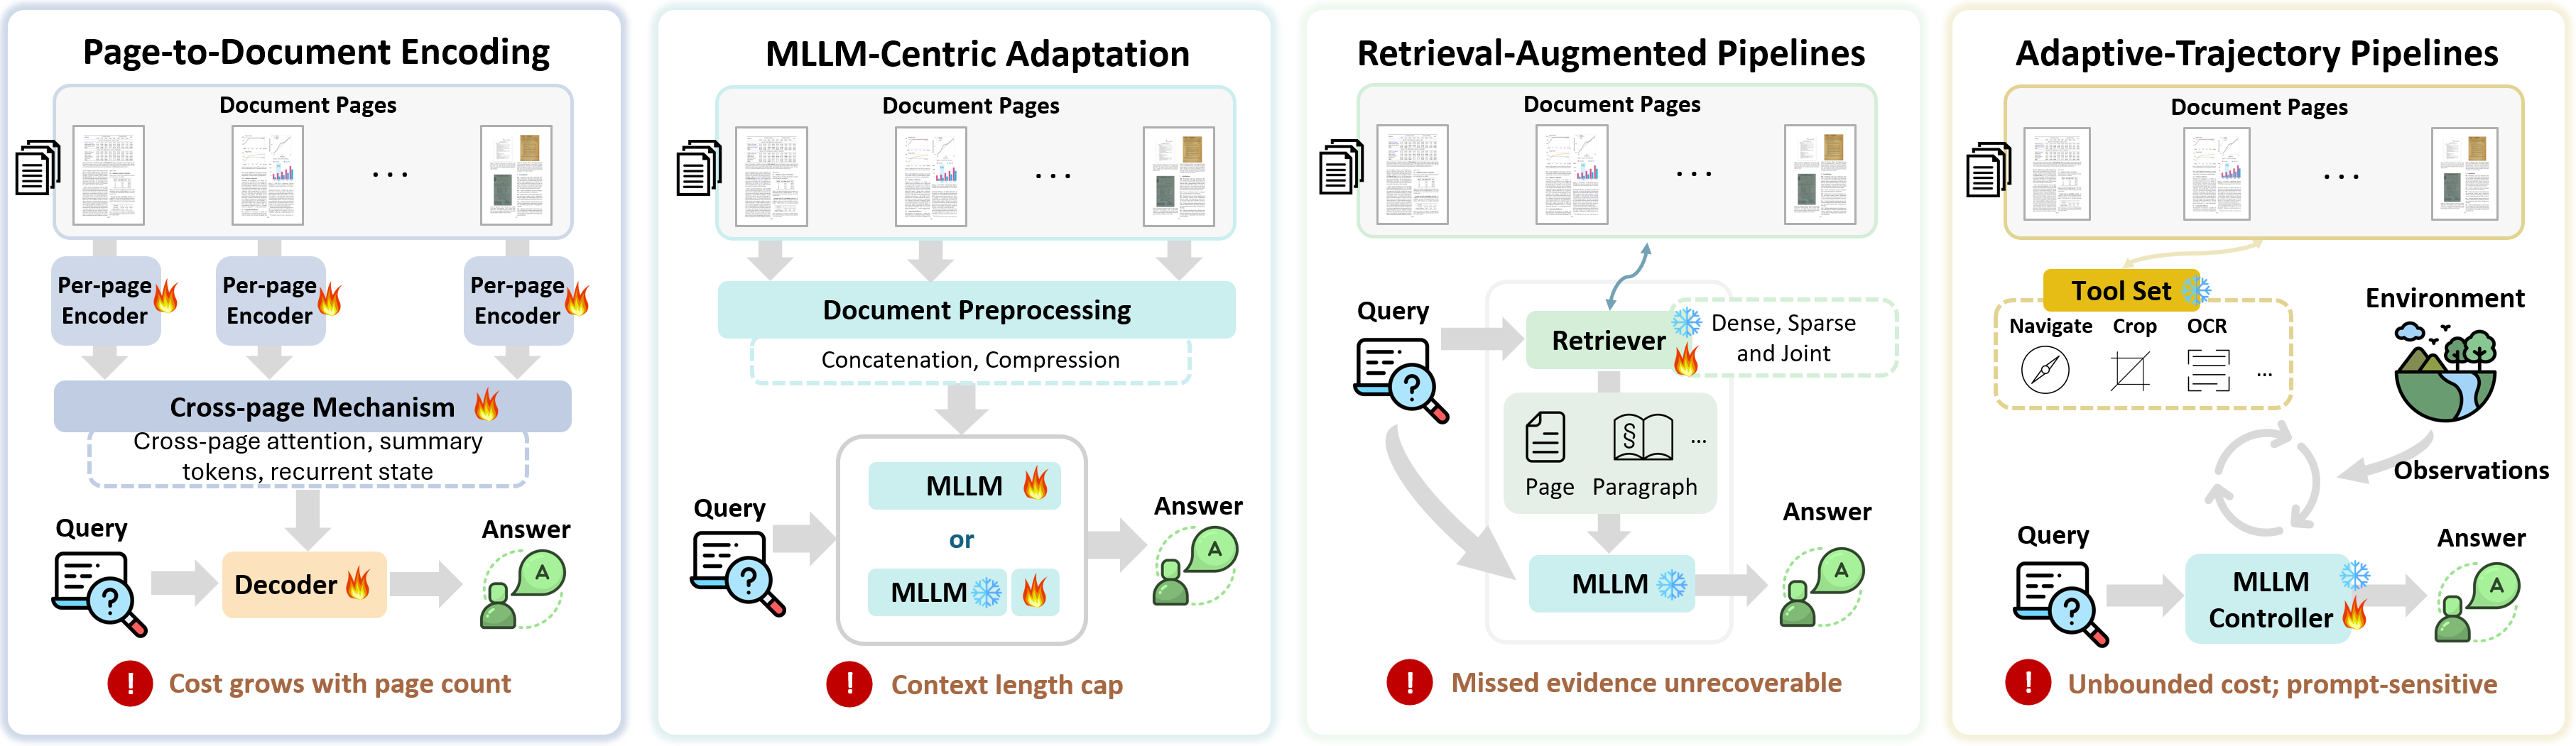
\includegraphics[width=\textwidth]{figures/mpvrdu_architecture.png}
    \caption{Illustration of MP-VRDU Architectures. Snowflake indicates component typically frozen; flame indicates component typically trained; both indicates even split across surveyed architectures.}
    % \emoji{snowflake} indicates component typically frozen; \emoji{fire} indicates component typically trained; \emoji{snowflake}\emoji{fire} indicates even split.}
    \label{fig:architecture}
\end{figure*}

\section{MP-VRDU Architecture Overview}
\label{sec:architecture}
The defining problem in MP-VRDU is evidence management: how a system manages cross-page evidence that is sparse, distributed, and frequently larger than any MLLM's context window, so a system must decide what to retain, discard, or retrieve. These decisions are determined by architectural design, which fixes \textbf{how evidence is selected, preserved, and exposed for reasoning}, and we therefore organise the field by architecture rather than by the OCR dependency used in prior surveys~\citep{ding2025survey}.
\textit{Page-to-document encoding models} jointly encode pages with cross-page representations (\S\ref{sec:arch-p2d}).
\textit{MLLM-centric adaptation models} adapt MLLMs to multi-page inputs within context and token budgets (\S\ref{sec:arch-mllm}).
\textit{Retrieval-augmented pipelines} retrieve relevant evidence before generation (\S\ref{sec:arch-ra}).
\textit{Agentic pipelines} iteratively inspect evidence using an LLM controller (\S\ref{sec:arch-agent}). Reported performance across the four families on principal MP-VRDU benchmarks is provided in Appendix~\ref{app:performance} (Table~\ref{tab:model_performance_arch}).
% Two trends emerge, distinguished by where the document resides at inference, and each divides into two families. \textbf{In-context encoding} holds the whole document within a single model's forward pass, covering page-to-document encoding models (\S\ref{sec:arch-p2d}) and backbone-centric adaptation models (\S\ref{sec:arch-mllm}). \textbf{Selective evidence pipelines} instead pass only a compact evidence subset to a generator, covering retrieval-augmented (\S\ref{sec:arch-ra}) and agentic pipelines (\S\ref{sec:arch-agent}). %The two trace a broadly chronological shift from encoding all pages jointly toward selectively retrieving and iteratively inspecting evidence.

\subsection{Page-to-Document Encoding Models}
\label{sec:arch-p2d}
Page-to-document encoding models process each page through a shared layout-aware encoder such as LayoutLMv3~\cite{huang2022layoutlmv3}, that fuses OCR text, bounding-box layout, and visual features within the page, then connect per-page representations through a cross-page exchange mechanism in a single forward pass~\cite{dong2024multi, borchmann2025arctic}. By preserving page boundaries and cross-page relations within the architecture, this design provides a strong inductive bias for documents with regular structural templates. However, joint encoding caps total document length at the encoder's capacity, and page-to-document compression discards fine-grained evidence as input grows, restricting this family's applicability to documents of shorter length.

\subsection{MLLM-Centric Adaptation Models}
\label{sec:arch-mllm}
MLLM-centric adaptation models process the document inside a pre-trained MLLM whose context window absorbs cross-page information directly, with adaptation ranging from training only lightweight modules to fine-tuning the backbone itself~\cite{tanaka2024instructdoc, hu2025mplug2, duan2025docopilot, xiong2026docr1}. This design benefits directly from the MLLM's instruction-following and reasoning capabilities. However, the backbone's context length caps total document size, fine-grained signals depend on the fidelity of token compression~\cite{jia2024leopard}, and document structure must be recovered implicitly from the input~\cite{hannan2025docslm}.

\subsection{Retrieval-Augmented Pipelines}
\label{sec:arch-ra}
Retrieval-augmented pipelines decouple evidence selection from answer generation: a retriever first selects relevant evidence units, such as chunks, pages, or graph nodes, and the generator then produces an answer conditioned on this compact subset~\cite{cho2024m3docrag, tanaka2025vdocrag}.  This family spans single-pass retriever-generator systems~\cite{cho2024m3docrag} to multi-component pipelines that compose multiple LLM-instantiated ``agents'' in specialised roles~\cite{han2025mdocagent, suri2025visdom}, all of which follow trajectories fixed at design time. As such, inference cost is bounded, and by passing only selected evidence to the generator, these pipelines scale to longer documents. However, evidence missed during retrieval is unrecoverable at generation, making retriever recall the binding constraint on this family, and upstream errors in chunking, OCR, or modality alignment propagate directly to the final answer.

% If want to go with agentic, could name it "Adaptive-Agent Pipelines"
\subsection{Adaptive-Trajectory Pipelines}
\label{sec:arch-agent}
Adaptive-trajectory pipelines instantiate the agent paradigm of \citeauthor{plaat2025agentic} and \citeauthor{wang2024survey}, in which an LLM controller reasons, interacts with an external environment, and conditions subsequent actions on observed outcomes. Unlike the fixed ``agents'' of \S\ref{sec:arch-ra}, the controller's trajectory is not predetermined, rather, it selects each evidence-gathering action at inference time~\cite{zheng2026docvstar, sun2025docagent}, with actions surfacing as calls to external tools~\cite{wang2025vidorag, yu2025mact} or as navigation over a pre-built document representation~\cite{jain2025simpledoc, fu2026dmap}. ReAct~\cite{yao2022react} is the most common controller realisation (see \S\ref{sec:agentic-methods}), though iterative-reflection variants also appear. The cost of this flexibility is controllability: variable-length trajectories make inference cost hard to bound and controllers may commit early to wrong evidence with silent failure, but the trade-off is worthwhile, since unbounded cost is recoverable through engineering whereas missed evidence is not.

%The cost of this flexibility is controllability: variable-length trajectories make inference cost hard to bound, controllers may commit early to wrong evidence with silent failure, and the system still inherits the recall ceiling of every tool used.

\section{Multi-Page Multimodal Representation}
\label{sec:modality}
Every evidence-management decision is enacted over a specific modality, and its cost depends on how that modality is represented under the tension between page coverage and reading fidelity. This section reviews text (\S\ref{sec:modality-text}), visual (\S\ref{sec:modality-visual}), and cross-page structural (\S\ref{sec:modality-structure}) modelling under this pressure; fusion is deferred to Appendix~\ref{app:fusion}.

\subsection{Text Modality}
\label{sec:modality-text}
Text in MP-VRDU presents four bottlenecks. \textbf{Volume} across pages frequently exceeds the MLLM context, addressed by aggressive compression into a fixed budget~\cite{borchmann2025arctic, dong2024multi}, by native long-context training that widens the input window~\cite{duan2025docopilot}, or by indexing chunks and passing only selected text to the reader~\cite{xie2024wukong, zhang2024cream}; each shifts the lossy choice to a different stage. \textbf{Continuity} breaks when paragraphs, tables, and sections span page boundaries; it is preserved through document-level layers over per-page representations~\cite{tito2023hierarchical, blau2024gram} or structure-aware chunking and adjacent-page expansion at retrieval time~\cite{shin2025multidocfusion, qian2026accurate}, each restoring local context at the cost of token-level detail or query relevance. \textbf{Noise} compounds as OCR errors accumulate across the document, dampened upstream through layout-aware pipelines or downstream by treating low-confidence tokens as soft cues~\cite{hannan2025docslm}, yet propagation through retrieval indexes remains uncharacterised. \textbf{Heterogeneity} in text density receives the least attention, with adaptive page selection~\cite{li2025avir} the rare question-conditioned exception in a setting otherwise dominated by fixed-budget allocation.

\subsection{Visual Modality}
\label{sec:modality-visual}
Visual evidence preserves signals text extraction loses, but its computational cost introduces three bottlenecks. \textbf{Resolution} cannot be maintained at full document length, since token cost scales super-linearly under dynamic cropping~\cite{zheng2026docvstar}; it is managed by token-reduction modules that keep every page available at lower fidelity~\cite{hu2025mplug2, yu2024texthawk2, jia2024leopard}, thumbnail-based browsing with selective high-resolution inspection~\cite{zheng2026docvstar, jain2025simpledoc}, or high-fidelity reading of only retrieved pages that inherits the selector's recall ceiling~\cite{zhu2025doclens, yan2025docseeker}. \textbf{Multi-signal competition} forces text-bearing pixels, non-textual evidence, and layout cues to share one per-page budget; visual RAG retains patch-level granularity but ranks by layout similarity rather than answer-region confirmation~\cite{cho2024m3docrag, tanaka2025vdocrag}, element-level cropping preserves fine structure at the cost of detector dependence~\cite{zhu2025doclens}, and OCR-augmented visual reading delegates text recovery so the visual budget can prioritise non-textual evidence~\cite{hannan2025docslm}. \textbf{Heterogeneity} from varying visual complexity remains underexplored; evidence-guided allocation~\cite{yan2025docseeker} is one of the few question-conditioned approaches.

\subsection{Structure Modality}

\label{sec:modality-structure}
Structure turns isolated page observations into document evidence. Per-token layout remains relevant at MP scale~\cite{zhu2025laytokenllm}, but the MP-distinctive difficulty is structural relations whose scope crosses pages. \textbf{Hierarchy} is the foundational problem, since sections, headings, and reading order organise the document as a whole rather than any individual page. Explicit parsers recover this as outlines or hierarchical indices~\cite{shin2025multidocfusion, sun2025docagent, fu2026dmap}, OCR-free backbones learn it end-to-end from page images~\cite{hu2025mplug2}, and per-segment layout tokens encode each region's spatial arrangement without adding tokens to the context~\cite{zhu2025laytokenllm}. \textbf{Cross-page references} demand resolving pointers such as ``see Figure 3'' to their referents on other pages, rather than ranking by surface similarity; graph- and map-based methods represent these references as edges between document elements~\cite{wu2025molorag, fu2026dmap}, at the cost of edge quality bounded by extraction heuristics. \textbf{Spanning elements} such as multi-page tables and continued paragraphs require representations that bridge page boundaries without conflating distant content~\cite{gong2025mhier, qian2026accurate}.

\section{Inference-Time Adaptation Strategies}
\label{sec:inference-time}
Inference-time adaptation improves MP-VRDU performance by reshaping the inference pipeline around a frozen MLLM backbone rather than modifying its parameters. This makes it particularly suited to MP-VRDU, where supervised data is scarce and backbones must remain exchangeable across document types. We organise these strategies by the evidence-management decision they implement: selecting evidence (\S\ref{sec:tf-retrieval}), reasoning over assembled evidence (\S\ref{sec:tf-reasoning}), and iteratively acquiring further evidence (\S\ref{sec:agentic-methods}).

\subsection{Retrieval and Navigation}
\label{sec:tf-retrieval}
Retrieval narrows long documents to compact evidence units for downstream reasoning. Existing methods either rank evidences independently by query \textit{similarity} or traverse \textit{relation-aware} structures such as section hierarchies and cross-reference graphs.

\paragraph{Similarity-based Retrieval.}
\label{sec:similarity-based}
Similarity-based retrieval scores evidences independently against the query and returns the top-ranked subset. Sparse lexical signals such as BM-25 serve as baselines or auxiliary channels, while dense retrieval in MP-VRDU typically uses vision-language late-interaction encoders such as ColPali and ColQwen that align token-level query vectors with patch-level page embeddings, preserving fine-grained alignment between query terms and page regions~\cite{cho2024m3docrag, jain2025simpledoc}. Granularity varies from chunks to whole pages, with adaptive selectors adjusting the per-query retrieval count when evidence density is uneven~\cite{li2025avir}. A second reranking stage commonly refines an initial dense recall through LLM-based scoring over candidate evidences or page summaries, optionally under persistent working memory that carries cross-query context across iterations~\cite{zhang2024cream,xu2026mmr5}. Independent scoring handles paraphrase and cross-modal queries well, but cannot follow cross-page references or multi-hop dependencies that no single passage carries.

\paragraph{Relation-aware Retrieval.}
Relation-aware methods retrieve along explicit document structure rather than scoring evidences independently against the query. Tree-based variants extract section hierarchies and outlines, grouping evidences along semantic boundaries so retrieved chunks preserve parent context, with some routing queries through dual in-page and cross-page indices to recover both local and global evidence~\cite{shin2025multidocfusion, sun2025docagent, gong2025mhier}. Graph-based variants treat headings, entities, and cross-references as graph nodes with typed edges, allowing controllers to traverse from one passage to related ones rather than relying on similarity alone; extensions add logical relevance scoring or query-conditioned graph construction to bias traversal toward inferentially connected nodes~\cite{wang2024knowledge, wu2025molorag, zhang2026mldocrag}. Structure-based methods recover evidence links that similarity scoring misses, at the cost of dependence on parser quality and traversal cost that grows with the multi-hop count required to answer the question.

\subsection{Prompted Reasoning Strategies}
\label{sec:tf-reasoning}
Prompted reasoning strategies act over a single evidence buffer assembled prior to the reasoning call, which may be the full document representation, a retrieved subset, or evidence from an agentic step. We cover the four mainstream prompting paradigms; the coarse-to-fine pattern that recurs across many surveyed systems is treated separately in Appendix~\ref{app:coarse-to-fine}.

\paragraph{Sequential Reasoning.}
A single reasoning thread proceeds linearly, optionally with revision. \emph{Chain-of-Thought (CoT)}~\cite{wei2022chain} is widely adopted in MP-VRDU to bind evidence from different pages step by step and decompose multi-hop questions into single-hop steps~\cite{jia2024leopard, xu2026mmr5}, but operates only over the assembled evidence, locating its contribution in the fidelity rather than the recall stage of the pipeline. \emph{Self-Reflection} (Reflexion-style)~\cite{shinn2023reflexion} extends the single thread with iterative revision against a verifier or critic~\cite{jain2025simpledoc, wang2025vidorag}, reducing single-pass error at the cost of additional rounds and a self-evaluation signal whose reliability bounds the gains.

\paragraph{Parallel Exploration.}
Multiple reasoning paths are produced in parallel and combined into a single answer. \emph{Self-Consistency}~\cite{wang2022self} samples multiple chains and selects the majority answer, with sampling-adjudication variants replacing the vote with an LLM judge~\cite{zhu2025doclens}, scaling robustness with inference cost. \emph{Tree-of-Thoughts (ToT)}~\cite{yao2023tree} explores reasoning branches with backtracking, but has seen limited uptake in MP-VRDU, where evidence sparsity rather than search-space branching is the dominant difficulty.

\subsection{Agentic Methods}
\label{sec:agentic-methods}
Agentic methods distribute the MP-VRDU workflow across one or more LLM-instantiated controllers, either iterating evidence acquisition under inference-time control or coordinating across specialised roles. We note that \textit{agentic} is used ambiguously in the MP-VRDU literature, covering both systems whose controller selects actions at inference time, following the framing by \citeauthor{plaat2025agentic} and \citeauthor{wang2024survey}, and systems composed of multiple LLM-instantiated agents in fixed roles; we treat both senses here, following the architectural distinction in \S\ref{sec:arch-ra}–\S\ref{sec:arch-agent}.

\paragraph{ReAct and Tool-Augmented Reasoning.}
ReAct prompting~\cite{yao2022react} augments the action space with language thoughts, interleaving thought-action emissions in a single stream whose observations feed the next step, letting a single controller acquire evidence during inference rather than reasoning over a fixed buffer. The action space takes two forms in MP-VRDU. Document-side tool calls invoke external retrievers, parsers, or OCR engines, with each round concentrating on a chosen page or region~\cite{sun2025docagent, wu2025docreact}, lifting the single-step recall ceiling of retrieval-augmented pipelines. Structured navigation instead operates over a pre-built document representation (see \S\ref{sec:modality-structure}), with the controller selecting which node, section, or page to inspect next~\cite{zheng2026docvstar}. Adaptive-trajectory systems that lack the thought-action schema, such as those built on Reflexion-style iterative refinement~\cite{jain2025simpledoc, fu2026dmap}, share the iterative control regime without being ReAct in the strict sense. 
%Tool latency, compounding error from early wrong actions, and unbounded trajectory length remain shared limitations.

\paragraph{Multi-Agent Orchestration.}
Multi-agent orchestration distributes the workflow across multiple controllers whose interaction pattern, rather than a single monolithic controller, drives evidence gathering and answer synthesis. Each controller operates on a narrower input and clearer objective than a single backbone tasked with the entire workflow, mitigating the cognitive overload that arises when one model must locate, read, verify, and answer over the entire document~\cite{yu2025mact}. Two patterns recur. \textit{Modality-specialised} decomposition assigns separate controllers to text and visual evidence and adds a synthesis controller that reconciles their outputs, preserving single-modality reading fidelity at the cost of a reconciliation step that lacks access to the original document~\cite{han2025mdocagent, duan2025m2rag}. \textit{Role-specialised} decomposition assigns controllers to procedural stages such as planning, execution, verification, and synthesis, with routing between stages when a downstream controller detects an error~\cite{yu2025mact, sun2025docagent}. Separating judgement from generation reduces the cognitive blind spots of self-correction, but introduces inter-controller compatibility costs and a recall ceiling bounded by upstream stages.

% Note on training: pretraining/continued-pretraining is rarely done in MP-VRDU, mostly SFT and IT for training trajectory, reasoninig, orchestration etc.
\section{Training Strategies}
\label{sec:training}
Training internalises the evidence-management decisions of \S\ref{sec:inference-time} into model parameters, supplying capabilities that prompting cannot: cross-page evidence selection (\S\ref{sec:train-retrieval}), document-scale reasoning over assembled evidence (\S\ref{sec:train-reasoning}), and reliable agentic acquisition (\S\ref{sec:train-agentic}). Two cross-cutting techniques recur across all three (\S\ref{sec:train-crosscutting}).

\subsection{Trained Retrieval Components}
\label{sec:train-retrieval}
Off-the-shelf encoders such as ColPali and ColQwen~\cite{Faysse2024-wq} score each page independently, leaving retrieval dominated by local query-page similarity rather than document-level context. Retriever training has therefore explored three complementary directions. \textbf{Modality-alignment} methods align visual page embeddings with OCR-derived text representations, enabling page-image retrieval without late-interaction scoring at inference~\cite{tanaka2025vdocrag}, trading index size for query-time efficiency. \textbf{Cross-page-fusion} methods enrich each page representation with neighbouring-page context~\cite{qian2026accurate}, recovering distributed evidence without rebuilding the encoder, though the optimal neighbour window is corpus-dependent and rarely tuned per query. \textbf{Logical-relevance} methods train graph-based scorers that rank pages by their position in cross-page reasoning paths rather than embedding similarity~\cite{wu2025molorag}, addressing multi-hop questions whose evidence pages are individually low-scoring at the cost of inheriting the graph-extractor's failure modes. The three directions are not interchangeable: modality-alignment improves throughput, cross-page-fusion improves recall on adjacent evidence, and logical-relevance improves recall on inferentially-connected evidence.

\subsection{Trained Reasoning Methods}
\label{sec:train-reasoning}
Prompted reasoning leaves quality sensitive to prompt design and base-model behaviour, motivating training that internalises reasoning patterns into the backbone. \textbf{Trace-imitation} variants supervise the backbone on demonstration chains wrapped in fixed schema tags such as \texttt{<think>}, \texttt{<evidence>}, and \texttt{<answer>}~\cite{yan2025docseeker, guo2026end}, which provides structure that downstream verifiers can audit but inherits any biases or omissions in the teacher's chains. \textbf{Reward-driven} variants optimise the reasoning policy with Group Relative Policy Optimisation (GRPO) against rewards combining answer accuracy, evidence-page recall, and format compliance~\cite{xiong2026docr1, xu2026mmr5}, typically warm-started from a trace-imitation stage; the two are therefore sequential rather than alternative, with reward-driven training refining what imitation alone cannot. \textbf{Uncertainty-calibration} variants learn an aggregation head that selects across candidate outputs by calibrated uncertainty~\cite{hannan2025docslm}, providing a learned self-consistency signal without test-time chain sampling, which suits parameter or compute budgets that preclude sampling-based approaches.

\subsection{Trained Agentic Methods}
\label{sec:train-agentic}
Prompt-only agentic control is unreliable on smaller open-weight backbones, which cannot consistently follow ReAct schemas and select among tool calls. \textbf{Trajectory-distillation} variants clone agentic trajectories from a stronger teacher through SFT on think-action-observation turns~\cite{zheng2026docvstar, zhang2026docdancer}, with closed-loop teacher collection essential because retrieval and fetching change subsequent observations; distillation is bounded by teacher quality and inherits the teacher's blind spots. \textbf{Reinforcement-learned} variants optimise the agentic policy directly against trajectory-level rewards combining answer correctness, evidence recall, and tool-use shape~\cite{wang2026vragrl, lin2026mmdocr1}, lifting the teacher-quality ceiling at the cost of training instability that multi-turn variants address through entropy-based stopping, similarity-weighted baselines, or per-role budget allocation. The surveyed evidence does not cleanly separate the two, since reported comparisons confound the training objective with backbone, reward design, and trajectory budget.

\subsection{Cross-Cutting Training Techniques}
\label{sec:train-crosscutting}
Two techniques recur across retriever, reasoner, and agent training. \textbf{Parameter-efficient tuning} (PEFT) is dominant: full backbone fine-tuning is prohibitive at long-document context lengths and risks erasing pretrained capabilities, so the prevailing pattern freezes the backbone and trains lightweight modules through Low-Rank Adaptation (LoRA), projection heads, or task-specific adapters~\cite{zhang2024cream, qian2026accurate, zhang2026docdancer}, with the choice of module driven more by compute budget than by target component. \textbf{Multi-stage curriculum training} addresses a different concern: several systems start on single-page objectives before introducing document-scale supervision~\cite{hu2025mplug2, hannan2025docslm, xiong2026docr1}, exploiting the fact that text reading and layout understanding transfer from single-page data while cross-page integration must be learned separately. Their recurrence across dissimilar systems indicates that cross-page integration does not emerge from single-page supervision alone.

\section{Datasets}
\label{sec:datasets}
Multi-page documents impose a structural constraint absent from the single-page setting: per-page annotation does not scale, and multi-page corpora are scarce because long PDFs are harder to source, license, and parse than single pages. This constraint shapes all three dataset roles in MP-VRDU differently from SP-VRDU. \textbf{Pretraining} is the exception rather than the norm, confined to a few page-to-document and MLLM-centric systems that perform continued pretraining on existing backbones, since multi-page pretraining corpora remain small relative to the single-page archives that preceded them. \textbf{Fine-tuning} has converged on LVLM-synthesised supervision over scraped PDFs, with reinforcement learning increasingly layered on top to shape evidence-grounding and trajectory behaviour rather than to scale the data itself. \textbf{Benchmarking} has stratified into three tiers: single-page extractive baselines, mid-length multi-page suites, and long-document multimodal benchmarks requiring cross-page integration, with retrieval and page-localisation increasingly scored alongside answer accuracy. The same scarcity of source documents that drives synthetic generation also concentrates fine-tuning and evaluation onto the same small pool of PDFs, a contamination risk we return to in \S\ref{sec:challenges}. For full details see Appendix~\ref{app:dataset-details}.

\section{Challenges and Future Work}
\label{sec:challenges}
A consistent pattern emerges across MP-VRDU systems: progress comes from moving evidence handling out of the backbone, through compression, retrieval, or iterative orchestration, but each shift relocates the bottleneck rather than removing it. Five challenges define the open frontier: three concern system capability (the evidence pipeline itself, faithfulness, and efficiency) and two concern data and evaluation (supervision integrity and evaluation scope).
\paragraph{Evidence Pipeline Bottleneck.}
\label{sec:evidence}
MP-VRDU systems must reconcile high-resolution per-page reading with document-scale evidence aggregation, an objective that exceeds any MLLM's compute and context budget~\cite{ma2024mmlongbench}. Every architectural family takes a lossy compromise: compression silently drops fine-grained content and is typically fixed before the question is seen; retrieval bounds answer accuracy from above while broader retrieval introduces attention dilution; and iterative retrieval lifts this ceiling only partially, inheriting the recall of every tool it calls. Cross-page structure compounds this further, as none of the routes in \S\ref{sec:modality-structure} scales cleanly. Future work should explore query-conditional compression, retrieval that follows cross-references and logical relations, and learned cross-page structural representations.

\paragraph{Faithfulness and Abstention.}
\label{sec:faithfulness}
Long documents amplify hallucination risk; when retrieval misses or compression discards the answer-bearing region, current systems still produce confident answers. Few surveyed systems support abstention, calibrated uncertainty, or citation-grounded generation, leaving downstream users without signals to distinguish supported answers from fabrications. Future work should integrate evidence-grounded decoding, learned abstention against unanswerable or unretrievable questions, and trajectory-level faithfulness audits that verify the cited evidence supports the final answer.

\paragraph{Efficiency and Deployability.}
\label{sec:efficiency}
Agentic and retrieval-augmented pipelines routinely issue tens of LLM calls per question, with token costs scaling jointly with document length and trajectory length. The surveyed literature reports almost no inference-cost analysis: end-to-end latency, token budgets per query, and accuracy–cost Pareto curves are largely absent, despite their centrality to enterprise deployment. Future work should treat compute as a first-class evaluation axis, develop efficient inference techniques specific to long documents such as cross-round caching, speculative decoding, and adaptive depth, and explore compact MP-VRDU models~\cite{hannan2025docslm} that operate under realistic on-device or privacy constraints.

\paragraph{Supervision Scarcity and Contamination.}
\label{sec:supervision}
Per-page annotation does not scale to documents averaging tens of pages, so most systems rely on LVLM-synthesised QA over scraped PDFs~\cite{tanaka2024instructdoc, jain2025simpledoc, xiong2026docr1, zhang2026docdancer}. Compounding this, benchmark construction often reuses documents from earlier suites: MMLongBench-Doc draws documents from DUDE, SlideVQA, and ChartQA~\cite{ma2024mmlongbench}, while MP-DocVQA is built on DocVQA~\cite{tito2023hierarchical, mathew2021docvqa}. Together, MLLM-generated QA data~\cite{deng2025longdocurl} and benchmark-reused fine-tuning sets~\cite{xiong2026docr1, duan2025docopilot} risk contamination: models may train on benchmark-derived documents and be evaluated on overlapping data, sometimes judged by the same MLLM family. Future work should adopt held-out documents, declare cross-suite overlap, and separate generators from evaluators. More details and overlap matrix available in Appendix~\ref{app:contamination}.

\paragraph{Evaluation Methodology and Scope.}
\label{sec:evaluation}
Beyond contamination, two further evaluation gaps persist. Answer-only accuracy masks retrieval failure and rewards correct answers reached through incorrect reasoning; newer benchmarks score retrieval and page-localisation alongside VQA-style answers~\cite{hui2024uda, xiong2026docr1, zhu2025doclens}, but the practice is not yet standardised, and agentic pipelines produce stochastic trajectories that further complicate reproducibility. Task, language, and domain scope also remain narrow. Real-world MP-VRDU spans summarisation and structured extraction beyond VQA, multilingual layouts beyond English, and domain-specialised settings such as medical, legal, and financial documents, as well as streaming inputs that arrive page-by-page. These dimensions are inherited from SP-VRDU~\cite{ding2025survey} rather than introduced by the multi-page setting and remain underexplored in both regimes. Future work should therefore standardise trajectory-level evaluation with retrieval and grounding metrics, report stochasticity bounds, and broaden coverage along these inherited dimensions.

\newpage

\section*{Limitations}
This survey covers multi-page VRDU models published before May 2026 and is bounded by the rapid pace of the field, with new architectures, training-free methods, and benchmarks appearing during preparation that may not be reflected here. Selection prioritises representative coverage of architectural and inference-time strategies over exhaustive enumeration. Cross-model performance comparisons are inherently limited since training distributions, benchmark coverage, and evaluation metrics are bespoke per system, and quantitative claims should be interpreted as indicative rather than definitive.

\section*{Acknowledgements}
This research was supported by the Australian Research Council (ARC) Training Centre for Critical Resources for the Future (CCRF) under grant number IC230100035.
% Bibliography entries for the entire Anthology, followed by custom entries
%\bibliography{anthology,custom}
% Custom bibliography entries only
\bibliography{custom}

\clearpage 

\newpage
\appendix

% ─────────────────────────────────────────────────────────────────────────────
% MP-VRDU Survey Taxonomy Figure
%
% Required packages (add to your preamble if not already present):
%   \usepackage{tikz}
%   \usepackage{forest}
%   \usepackage{xcolor}
%   \usepackage{adjustbox}
%   \usetikzlibrary{arrows.meta}
% ─────────────────────────────────────────────────────────────────────────────

% ── Column widths — edit these to resize boxes per column. ───────────────────
% If the text exceeds the width, it will wrap onto a second (or third) line.
\newcommand{\TaxRootWidth}{30mm}
\newcommand{\TaxSectionWidth}{16mm}
\newcommand{\TaxSubsectionWidth}{34mm}
\newcommand{\TaxIdeaWidth}{26mm}
\newcommand{\TaxLeafWidth}{63mm}


% ── Spacing parameters. ──────────────────────────────────────────────────────
% \TaxEdgeStub: length of the horizontal stub leaving each parent box before
% the edge turns vertical. Increase if the perpendicular gap looks too small.
\newcommand{\TaxLevelSep}{14pt}
\newcommand{\TaxSiblingSep}{1.2pt}
\newcommand{\TaxEdgeStub}{6pt}

% ── Colours — edit to recolour the figure. ───────────────────────────────────
\definecolor{nodebg}{HTML}{E8E8E8}
\definecolor{leafbg}{HTML}{D6E6F4}

\begin{figure*}[p]
\centering
\begin{adjustbox}{max totalsize={\textwidth}{0.92\textheight},center}
\begin{forest}
  for tree={
    grow'=east,
    parent anchor=east,
    child anchor=west,
    anchor=west,
    align=left,
    edge={-{Stealth[length=3pt]}, thin, gray!55},
    edge path={
      \noexpand\path[\forestoption{edge}]
        (!u.parent anchor) -- +(\TaxEdgeStub,0) |- (.child anchor)\forestoption{edge label};
    },
    l sep=\TaxLevelSep,
    s sep=\TaxSiblingSep,
    font=\scriptsize,
    rounded corners=2pt,
    draw=gray!50,
    inner sep=2.5pt,
    inner xsep=4pt,
    fill=nodebg,
  },
  % Root: rotated 90° banner. parent anchor=south puts the outgoing edge on
  % the visible east of the rotated box, so the line does not overlap the box.
  where level=0{
    font=\small\bfseries,
    align=center,
    rotate=90,
    anchor=center,
    parent anchor=south,
    text width=\TaxRootWidth,
  }{},
  % Section column.
  where level=1{font=\scriptsize\bfseries, text width=\TaxSectionWidth, align=left}{},
  % Subsection column.
  where level=2{text width=\TaxSubsectionWidth, align=left}{},
  % Idea column (level 3 non-leaf; level-3 leaves in §7/§8 fall through to leaf rule below).
  where level=3{text width=\TaxIdeaWidth, align=left}{},
  % Leaf rule comes LAST so it overrides any level-specific width above.
  % Applies to every node with no children (level 4 in §3–§6, level 3 in §7/§8).
  where n children=0{
    tier=leafrow,
    fill=leafbg,
    font=\tiny,
    text width=\TaxLeafWidth,
    align=left,
  }{},
  [MP-VRDU Taxonomy
    %% ── §3 Architecture ───────────────────────────────────────────────────
    [§\ref{sec:architecture}~Architecture
      [§\ref{sec:arch-p2d}~Page-to-Document
        [Summary tokens
          [{Hi-VT5~\cite{tito2023hierarchical}}]
        ]
        [Cross-page attention
          [{Arctic-TILT~\cite{borchmann2025arctic}, GRAM~\cite{blau2024gram}}]
        ]
        [Recurrent state
          [{RM-T5~\cite{dong2024multi}}]
        ]
      ]
      [§\ref{sec:arch-mllm}~MLLM-Centric
        [Lightweight projector
          [{InstructDoc~\cite{tanaka2024instructdoc}, LayTokenLLM~\cite{zhu2025laytokenllm}}]
        ]
        [Token compression
          [{mPLUG-DocOwl2~\cite{hu2025mplug2}, Texthawk2~\cite{yu2024texthawk2}}]
        ]
        [Backbone fine-tuning
          [{Docopilot~\cite{duan2025docopilot}, DocR1~\cite{xiong2026docr1}}]
        ]
      ]
      [§\ref{sec:arch-ra}~Retrieval-Augmented
        [Single retriever-reader
          [{M3DocRAG~\cite{cho2024m3docrag}, VDocRAG~\cite{tanaka2025vdocrag}}]
        ]
        [Multi-component pipeline
          [{MDocAgent~\cite{han2025mdocagent}, VisDoM~\cite{suri2025visdom}}]
        ]
      ]
      [§\ref{sec:arch-agent}~Adaptive-Trajectory
        [External tool calls
          [{ViDoRAG~\cite{wang2025vidorag}, MACT~\cite{yu2025mact}}]
        ]
        [Structured navigation
          [{SimpleDoc~\cite{jain2025simpledoc}, DMap~\cite{fu2026dmap}}]
        ]
      ]
    ]
    %% ── §4 Modalities ────────────────────────────────────────────────────
    [§\ref{sec:modality}~Modalities
      [§\ref{sec:modality-text}~Text
        [Volume
          [{Arctic-TILT~\cite{borchmann2025arctic}, PDF-WuKong~\cite{xie2026wukong}}]
        ]
        [Continuity
          [{RM-T5~\cite{dong2024multi}, MultiDocFusion~\cite{shin2025multidocfusion}}]
        ]
        [Heterogeneity
          [{AVIR~\cite{li2025avir}}]
        ]
      ]
      [§\ref{sec:modality-visual}~Visual
        [Resolution (compression)
          [{Texthawk2~\cite{yu2024texthawk2}, Leopard~\cite{jia2024leopard}}]
        ]
        [Selective high-res
          [{DocSeeker~\cite{yan2025docseeker}, DocLens~\cite{zhu2026doclens}}]
        ]
        [Multi-signal competition
          [{M3DocRAG~\cite{cho2024m3docrag}, VDocRAG~\cite{tanaka2025vdocrag}}]
        ]
      ]
      [§\ref{sec:modality-structure}~Structure
        [Hierarchy \& reading order
          [{DocAgent~\cite{sun2025docagent}, DMap~\cite{fu2026dmap}}]
        ]
        [Cross-page references
          [{KGP~\cite{wang2024knowledge}, MoLoRAG~\cite{wu2025molorag}}]
        ]
        [Spanning elements
          [{MHier-RAG~\cite{gong2025mhier}, DFVC~\cite{qian2026accurate}}]
        ]
      ]
    ]
    %% ── §5 Inference-Time Adaptation ─────────────────────────────────────
    [§\ref{sec:inference-time}~Inference
      [§\ref{sec:tf-retrieval}~Retrieval \& Navigation
        [Similarity-based
          [{ColPali~\cite{faysse2024colpali}, SimpleDoc~\cite{jain2025simpledoc}}]
        ]
        [Relation-aware
          [{MultiDocFusion~\cite{shin2025multidocfusion}, MLDocRAG~\cite{zhang2026mldocrag}}]
        ]
      ]
      [§\ref{sec:tf-reasoning}~Prompted Reasoning
        [Sequential Reasoning
          [{Leopard~\cite{jia2024leopard}, MM-R5~\cite{xu2026mmr5}}]
        ]
        [Parallel Exploration
          [{DocLens~\cite{zhu2026doclens}, ToT~\cite{yao2023tree}}]
        ]
      ]
      [§\ref{sec:agentic-methods}~Agentic Methods
        [ReAct \& tool-augmented
          [{Doc-V*~\cite{zheng2026docvstar}, Doc-React~\cite{wu2025docreact}}]
        ]
        [Modality-specialised
          [{MDocAgent~\cite{han2025mdocagent}, M$^2$RAG~\cite{duan2025m2rag}}]
        ]
        [Role-specialised
          [{MACT~\cite{yu2025mact}, DocAgent~\cite{sun2025docagent}}]
        ]
      ]
    ]
    %% ── §6 Training Strategies ───────────────────────────────────────────
    [§\ref{sec:training}~Training
      [§\ref{sec:train-retrieval}~Retrieval
        [Modality alignment
          [{VDocRAG~\cite{tanaka2025vdocrag}}]
        ]
        [Cross-page fusion
          [{DFVC~\cite{qian2026accurate}}]
        ]
        [Logical relevance
          [{MoLoRAG~\cite{wu2025molorag}}]
        ]
      ]
      [§\ref{sec:train-reasoning}~Reasoning
        [Trace imitation
          [{DocSeeker~\cite{yan2025docseeker}, CoR~\cite{guo2026end}}]
        ]
        [Reward-driven RL
          [{DocR1~\cite{xiong2026docr1}, MM-R5~\cite{xu2026mmr5}}]
        ]
        [Uncertainty calibration
          [{DocSLM~\cite{hannan2025docslm}}]
        ]
      ]
      [§\ref{sec:train-agentic}~Agentic
        [Trajectory distillation
          [{Doc-V*~\cite{zheng2026docvstar}, DocDancer~\cite{zhang2026docdancer}}]
        ]
        [Reinforcement-learned
          [{MM-Doc-R1~\cite{lin2026mmdocr1}, VRAG-RL~\cite{wang2026vragrl}}]
        ]
      ]
      [§\ref{sec:train-crosscutting}~Cross-Cutting
        [PEFT
          [{LayTokenLLM~\cite{zhu2025laytokenllm}, CREAM~\cite{zhang2024cream}}]
        ]
        [Multi-stage curriculum
          [{mPLUG-DocOwl2~\cite{hu2025mplug2}, DocSLM~\cite{hannan2025docslm}}]
        ]
      ]
    ]
    %% ── §7 Datasets (flattened: subsection → leaf) ───────────────────────
    [§\ref{sec:datasets}~Datasets
      [§\ref{app:dataset-pt}~Pretraining
        [{DocStruct4M~\cite{hu2024mplug}, MP-DocStruct1M~\cite{hu2025mplug2}}]
      ]
      [§\ref{app:dataset-sft}~Supervised Fine-tuning
        [{InstructDoc~\cite{tanaka2024instructdoc}, DocDancer~\cite{zhang2026docdancer}}]
      ]
      [§\ref{app:dataset-bm}~Benchmarking
        [{MMLongBench-Doc~\cite{ma2024mmlongbench}, LongDocURL~\cite{deng2025longdocurl}}]
      ]
    ]
    %% ── §8 Challenges (flattened: subsection → leaf) ─────────────────────
    [§\ref{sec:challenges}~Challenges
      [§\ref{sec:efficiency}~Efficiency \& Deployability
        [{DocSLM~\cite{hannan2025docslm}, URaG~\cite{shi2026urag}}]
      ]
      [§\ref{sec:faithfulness}~Faithfulness \& Abstention
        [{DocR1~\cite{xiong2026docr1}, DocLens~\cite{zhu2026doclens}}]
      ]
      [§\ref{sec:evidence}~Evidence Pipeline
        [{MHier-RAG~\cite{gong2025mhier}, KGP~\cite{wang2024knowledge}}]
      ]
      [§\ref{sec:supervision}~Supervision \& Contamination
        [{InstructDoc~\cite{tanaka2024instructdoc}, DocBench~\cite{zou2024docbench}}]
      ]
      [§\ref{sec:evaluation}~Evaluation Scope
        [{UDA~\cite{hui2024uda}, BRIDGE~\cite{xiang2026bridge}}]
      ]
    ]
  ]
\end{forest}
\end{adjustbox}
\caption{MP-VRDU Taxonomy}
\label{fig:taxonomy}
\end{figure*}


\section{More Methodology Details}
\label{app:methodology}

\paragraph{Search keywords.}
Queries combined a multi-page cluster with a task or method cluster. Multi-page terms included ``multi-page document'', ``long document'', ``long-context document'', ``cross-page reasoning'', ``page-level retrieval'', ``document-scale evidence'', and ``hundred-page''. Task and method terms included ``document visual question answering'', ``visually rich document understanding'', ``document VQA'', ``document agent'', ``visual document retrieval'', ``document RAG'', ``hierarchical document transformer'', and ``long-context vision-language model''. Benchmark-name probes (``MP-DocVQA'', ``MMLongBench-Doc'', ``LongDocURL'', ``DUDE'', ``SlideVQA'', ``M3DocVQA'', ``DocBench'', ``M-LongDoc'') were used as anchors for forward-citation sweeps to capture systems that report against multi-page evaluation suites.

\paragraph{Inclusion and exclusion criteria.}
A paper was retained if it (i) proposed a multi-page model, framework, system, or pipeline rather than a benchmark or dataset alone, and (ii) reported quantitative results on at least one multi-page benchmark, with cross-page evidence handling as an explicit design contribution. Excluded categories were single-page-only systems benchmarked solely on DocVQA, InfographicVQA, ChartQA, FUNSD, or CORD; survey, position, and opinion papers; generic OCR or table-extraction tools without VQA or reasoning evaluation; long-context LLM benchmarks where documents are one input type among many; and dataset-only contributions, which are catalogued separately in Appendix~\ref{app:dataset-details}. Peer-reviewed venue publications and arXiv preprints were assessed against the same substantive criteria, since recent MP-VRDU progress has appeared predominantly in preprint form; venue status is recorded per entry in Table~\ref{tab:model_survey_arch}.

\paragraph{Knowledge extraction and verification.}
Each retained paper was converted to markdown and processed through LLM-assisted key-information extraction with evidence-span location, populating per-model fields covering architectural family, OCR dependency, vision encoder, LLM backbone, adaptors and projectors, page-rendering resolution, training stages, datasets used per stage, and reported scores on each benchmark. Every extracted field was manually verified against the source paper before being committed to the corpus tables.

\paragraph{Dataset catalogue.}
The dataset catalogue in Appendix~\ref{app:dataset-details} was built primarily from the pretraining, fine-tuning, and benchmarking datasets named by every paper in the surveyed corpus, supplemented with a small set of datasets the corpus does not yet adopt but that cover MP-VRDU-relevant settings such as long scientific documents, multi-page tables, and cross-page reasoning suites, included to surface datasets whose adoption may strengthen future cross-system comparison.

\section{More Framework Details}
\label{sec:framework-details}

\subsection{Multimodal Fusion}
\label{app:fusion}
In multi-page VRDU, the central challenge is not only multimodal fusion itself, but determining when and how text, visual, and layout information should be selectively fused across large collections of pages under strict computational constraints.

\paragraph{Early Fusion.}
Text, visual, and layout features are combined before or during document encoding. In page-to-document transformers, fusion is local: OCR tokens, bounding boxes, visual patches, and question tokens are combined within each page and then aggregated through page summaries \cite{tito2023hierarchical}, document-level tokens \cite{blau2024gram}, recurrent memory \cite{dong2024multi}, or sparse text-image-layout attention \cite{borchmann2025arctic}. Backbone-centric MLLMs apply early fusion at projection time, mapping visual or multimodal features into the LLM token space through adapters, projectors, or document-former modules \cite{tanaka2024instructdoc, duan2025docopilot, jia2024leopard}. The pattern preserves fine-grained multimodal alignment at the cost of joint computation over many pages.

\paragraph{Late Fusion.}
Modalities are kept separate during retrieval or inspection and combined only after candidate evidence has been selected. Retriever-generator systems identify relevant evidences via text chunks before visual generation \cite{zhang2024cream}, perform page-image retrieval that keeps multimodal evidence fused at the page level \cite{cho2024m3docrag}, or combine parsed text, visual descriptions, parent pages, and cross-page summaries only for retrieved evidence \cite{gong2025mhier}. Agentic pipelines extend the pattern by inspecting text, image, table, and page-level evidence separately before final synthesis or adjudication \cite{han2025mdocagent, duan2025m2rag, zhu2025doclens}. The pattern scales to long documents but depends on retrieval and routing quality.

% Not that great, could omit entirely.
% \paragraph{Staged Fusion.}
% Local alignment is combined with selective document-level reasoning. Modalities are fused within pages or regions, then compressed, retrieved, or stored selectively before a final cross-page fusion step. Some hierarchical and recurrent models approximate the pattern by producing page-level summaries or memories prior to document-level aggregation \cite{tito2023hierarchical, dong2024multi}, and compact long-document models reduce local multimodal evidence into fixed-size page representations \cite{hannan2025docslm}. Fully developed staged fusion is rare in the surveyed corpus.

% % ─────────────────────────────────────────────────────────────────────────────
% Auto-generated by summary_models_convert.py — do NOT edit manually.
% Re-generate:  python3 summary_models_convert.py models_summary.csv models_summary.tex
%
% Required packages (add to your preamble):
%   \usepackage{booktabs}
%   \usepackage{longtable}
%   \usepackage{array}
%   \usepackage{xcolor}
%   \usepackage{colortbl}
%   \usepackage{caption}
%   \usepackage{adjustbox}   % for \begin{adjustbox}
%   \usepackage{natbib}      % for \citeyear  (or use biblatex)
%   \usepackage{lscape}      % optional: landscape
% ─────────────────────────────────────────────────────────────────────────────

\definecolor{sectionbg}{gray}{0.88}

% ── tab:model_survey_ocr ──────────────────────────────────────────────────────────────
\begin{table*}[t]
\centering
% \small
\scriptsize
\captionsetup{font=small}
\setlength{\tabcolsep}{3pt}
\renewcommand{\arraystretch}{0.86}
\begin{adjustbox}{width=\textwidth}
\begin{tabular}{l l c l l l c c c c}
\toprule
\textbf{Model} & \textbf{Venue} & \textbf{OCR Note} & \textbf{Architecture} & \textbf{Vision Encoder} & \textbf{LLM Backbone} & \textbf{Mod.} & \textbf{Reasoning} & \textbf{Search} & \textbf{Agentic} \\
\midrule

% ── OCR-Free ─────────────────────────────────────────────────────────────
\rowcolor{sectionbg}
\multicolumn{10}{l}{\textbf{OCR-Free}} \\
\midrule
  {Docopilot}~(\citeyear{duan2025docopilot}) & CVPR & Train & MLLM & InternViT-300M & Multiple (Intern) & V & - & - & - \\
  {DocR1}~(\citeyear{xiong2026docr1}) & AAAI & -- & MLLM & Qwen2.5-VL & Qwen2.5-VL-7B & V & CoT, HD & - & - \\
  {DocSeeker}~(\citeyear{yan2025docseeker}) & CVPR & -- & MLLM & Qwen2.5-VL ViT & Qwen2.5-VL-7B-Instruct & V & CoT, HD & - & - \\
  {Leopard}~(\citeyear{jia2024leopard}) & TMLR & -- & MLLM & SigLIP-SO400M & LLaMa-3.1-8B, Mistral-7B & V & CoT & - & - \\
  {mPLUG-DocOwl2}~(\citeyear{hu2025mplug2}) & ACL & -- & MLLM & ViT-L/14 & mPLUG-Owl2 & V & - & - & - \\
  {Texthawk2}~(\citeyear{yu2024texthawk2}) & preprint & Train & MLLM & SigLIP-SO400M & Qwen2-7B-Instruct & V & - & - & - \\
  {URaG}~(\citeyear{shi2026urag}) & AAAI & -- & MLLM & Qwen2.5-VL ViT & Qwen2.5-VL-3B / Qwen2.5-VL-7B & V & HD & - & - \\
  {AVIR}~(\citeyear{li2025avir}) & MMAsia & -- & RA & Pix2Struct & Qwen2.5-VL-3B-AWQ & V & - & D & 1A \\
  {DFVC}~(\citeyear{qian2026accurate}) & MDPI & -- & RA & VisRAG, ColQwen & Qwen2-VL-2B-Instruct & V & - & D & - \\
  {DREAM}~(\citeyear{zhang2025dream}) & MM & -- & RA & InternVL2 ViT & InternVL2-4B & V & HD & J & 1A \\
  {M3DocRAG}~(\citeyear{cho2024m3docrag}) & preprint & -- & RA & ColPali, ColQwen & Multiple (Qwen/Intern/Idefics) & V & - & D & 1A \\
  {MM-R5}~(\citeyear{xu2026mmr5}) & AAAI & -- & RA & Qwen2.5-VL ViT & Qwen2.5-VL-7B & V & CoT & D & - \\
  {MoLoRAG}~(\citeyear{wu2025molorag}) & EMNLP & -- & RA & ColPali & Multiple (Qwen/DS/LLaVA) & V & - & D, Nav & - \\
  {Self-Attention Scoring}~(\citeyear{kang2024multi}) & ICDAR & -- & RA & Pix2Struct & Pix2Struct & V & - & D & 1A \\
  {SLEUTH}~(\citeyear{liu2025sleuth}) & preprint & -- & RA & ColPali, Qwen3-VL ViT & Multiple (Qwen/GLM/Gemini) & V & HD & D & 4A \\
  {SV-RAG}~(\citeyear{chen2025svrag}) & ICLR & -- & RA & - & Multiple (Intern/Pali/Phi) & V & - & D & 1A \\
  {VDocRAG}~(\citeyear{tanaka2025vdocrag}) & CVPR & Train & RA & Phi3V-4.2B & Phi3V-4.2B & V & - & D & 1A \\
  {Doc-V*}~(\citeyear{zheng2026docvstar}) & preprint & -- & AT & Qwen2.5-VL & Qwen2.5-VL-7B-Instruct & V & ReAct, HD & D, IR, QR, Nav & 1A \\
  {DocReact}~(\citeyear{wu2025docreact}) & ACL & -- & AT & ColPali, VisRAG & GPT-4o & V & ReAct, QD & D, IR, QR & 1A \\
  {MACT}~(\citeyear{yu2025mact}) & preprint & -- & AT & Multiple & Multiple (Qwen/Intern) & V & CoT, PE & D & 4A, SC, SV \\
  {VRAG-RL}~(\citeyear{wang2026vragrl}) & NeurIPS & -- & AT & Qwen2.5-VL ViT & Qwen2.5-VL-3B/7B-Instruct & V & ReAct, HD & D, IR, QR & 1A \\

\midrule[0.4pt]

% ── OCR-Used ─────────────────────────────────────────────────────────────
\rowcolor{sectionbg}
\multicolumn{10}{l}{\textbf{OCR-Used}} \\
\midrule
  {Arctic-TILT}~(\citeyear{borchmann2025arctic}) & ACL & -- & PDE & U-Net & T5-Large & T, V, L & - & - & - \\
  {GRAM}~(\citeyear{blau2024gram}) & CVPR & -- & PDE & DocFormerv2 & DocFormerv2 & T, V, L & - & - & - \\
  {Hi-VT5}~(\citeyear{tito2023hierarchical}) & PR & -- & PDE & DiT & T5-Base & T, V, L & - & - & - \\
  {RM-T5}~(\citeyear{dong2024multi}) & DAS & -- & PDE & DiT & T5-Base & T, V, L & - & - & - \\
  {CoR}~(\citeyear{guo2026end}) & preprint & Aux. & MLLM & Qwen2.5-VL & Qwen2.5-VL-7B & T, V & CoT, PE, HD & - & - \\
  {DocSLM}~(\citeyear{hannan2025docslm}) & CVPR & -- & MLLM & SigLIP2 & Qwen2.5-1.5B & T, V, L & - & - & - \\
  {InstructDoc}~(\citeyear{tanaka2024instructdoc}) & AAAI & -- & MLLM & CLIP & FlanT5, BLIP2 & T, V, L & - & - & - \\
  {LayTokenLLM}~(\citeyear{zhu2025laytokenllm}) & CVPR & -- & MLLM & - & LLaMA3-8B, Qwen1.5-7B & T, L & - & - & - \\
  {CREAM}~(\citeyear{zhang2024cream}) & ACM & -- & RA & Pix2Struct & LLaMA2-7B & T, V & HD & J & 1A \\
  {KGP}~(\citeyear{wang2024knowledge}) & AAAI & -- & RA & - & Multiple & T, L & - & S, IR, Nav & 1A \\
  {M2RAG}~(\citeyear{duan2025m2rag}) & NeurIPS & Aux. & RA & VisRAG-Ret & Multiple (Qwen) & T, V & - & J & 3A \\
  {MDocAgent}~(\citeyear{han2025mdocagent}) & preprint & Aux. & RA & ColPali, ColQwen2 & Multiple (Llama/Qwen) & T, V & - & J & 5A \\
  {MHier-RAG}~(\citeyear{gong2025mhier}) & preprint & -- & RA & Qwen-VL-Plus & Multiple (Qwen/DS/GPT) & T, V, L & CoT, HD & J & 1A \\
  {MLDocRAG}~(\citeyear{zhang2026mldocrag}) & preprint & -- & RA & - & Multiple (Qwen) & T, V, L & CoT, HD & D & 1A \\
  {MultiDocFusion}~(\citeyear{shin2025multidocfusion}) & ACL & -- & RA & - & Multiple (Qwen/LLaMa/Mistral) & T, V, L & HD & D & 1A \\
  {PDF-WuKong}~(\citeyear{xie2024wukong}) & preprint & Aux. & RA & IXC2-VL-4KHD & IXC2-VL-4KHD & T, V & - & J & 1A \\
  {RAG-DocVQA}~(\citeyear{lopez2025enhancing}) & ICDAR & Aux. & RA & DiT, Pix2Struct & Qwen2.5-VL-7B-Instruct & T, V, L & - & D & 1A \\
  {VisDoMRAG}~(\citeyear{suri2025visdom}) & NAACL & Aux. & RA & ColPali / ColQwen2 & Multiple(Qwen/Gemini/GPT) & T, V & CoT & J & 3A, SC \\
  {DMAP}~(\citeyear{fu2026dmap}) & WWW & Aux. & AT & ColPali & GPT-4o / Qwen-plus & T, V, L & HD & J & 2A, SR \\
  {DocAgent}~(\citeyear{sun2025docagent}) & EMNLP & Aux. & AT & -- & Multiple (GPT/Gemini/Claude) & T, V, L & ReAct, HD & J, IR, Nav & 3A \\
  {DocDancer}~(\citeyear{zhang2026docdancer}) & preprint & Aux. & AT & Qwen3-VL-235B & Qwen3-4B/30B-A3B & T, V, L & ReAct & J, IR, QR & 1A \\
  {DocLens}~(\citeyear{zhu2025doclens}) & preprint & -- & AT & -- & Multiple (GPT/Gemini/Claude) & T, V, L & CoT & J & 4A, SA \\
  {MM-Doc-R1}~(\citeyear{lin2026mmdocr1}) & preprint & Aux. & AT & Qwen2.5-VL ViT & Qwen3-4B/8B & T, V & ReAct, HD & S, IR, QR, Nav & 3A \\
  {SimpleDoc}~(\citeyear{jain2025simpledoc}) & EMNLP & Aux. & AT & ColQwen-2.5 & Multiple (Qwen) & T, V & - & J, IR, QR & 1A, SR, SV \\
  {ViDoRAG}~(\citeyear{wang2025vidorag}) & EMNLP & Aux. & AT & NV-Embed-V2, ColQwen2 & Multiple (Qwen/LLaMa/GPT) & T, V & ReAct, HD & J, IR & 3A, SR, SV \\

\bottomrule
\end{tabular}
\end{adjustbox}
\caption{Survey of MP-VRDU models grouped by OCR dependency. PDE\,=\,Page-to-Document Encoding Models; MLLM\,=\,MLLM-Centric Adaptation Models; RA\,=\,Retriever-Augmented Pipelines; AT\,=\,Adaptive-Trajectory Pipelines. T\,=\,text; V\,=\,visual; L\,=\,layout. CoT\,=\,Chain of Thought; ReAct\,=\,Reason\,+\,Act; PE\,=\,Plan-Execute; QD\,=\,Question Decomposition; HD\,=\,Hierarchical / Coarse-to-Fine. S\,=\,Sparse; D\,=\,Dense; J\,=\,Joint; IR\,=\,Iterative Retrieval; QR\,=\,Query Reformulation; Nav\,=\,Navigation. $n$A\,=\,$n$ agents; SR\,=\,Self-Refine; SV\,=\,Self-Verify; SC\,=\,Self-Consistency; SA\,=\,Sampling-Adjudication. OCR Note column: Aux.\,=\,model is not strictly OCR-dependent but incorporates OCR as an auxiliary framework component; Train\,=\,OCR-derived supervision is used during training but no OCR is used at inference. `--' indicates not reported / not applicable.}
\label{tab:model_survey_ocr}
\end{table*}


% \subsection{Model Survey by OCR Dependency}
% \label{app:ocr-survey}
% Table~\ref{tab:model_survey_ocr} reorganises the surveyed systems along the OCR-dependency axis to complement the architectural grouping in Table~\ref{tab:model_survey_arch}. The two views cut across each other rather than nesting: OCR-using systems span every architectural family, and OCR dependency is therefore largely orthogonal to architecture rather than a defining feature, as discussed in \S\ref{sec:architecture}. The ``OCR Note'' column flags hybrid cases in which OCR appears only as an auxiliary component or during training.

\subsection{Coarse-to-Fine Reasoning}
\label{app:coarse-to-fine}
Coarse-to-fine reasoning is the most widely adopted structured-reasoning pattern in the surveyed corpus, appearing across MLLM-centric, retrieval-augmented, and adaptive-trajectory systems (Table~\ref{tab:model_survey_arch}). The pattern decomposes document-scale reasoning into successive stages of decreasing scope: an initial pass over the whole document or a broad candidate set identifies regions likely to contain answer-relevant evidence, and subsequent passes restrict attention to those regions at higher fidelity. Three implementations recur. \textbf{Page to region} variants first select candidate pages from the document, then reason over each candidate at higher fidelity or with more detailed analysis before answering~\cite{shi2026urag, xiong2026docr1, yan2025docseeker, gong2025mhier}, with some realisations operating across discrete passes and others embedding the pattern within the layers of a single MLLM. \textbf{Retrieve, rerank, then read} variants extend the pattern across the retrieval stack, with an initial dense or sparse retrieval returning a broad candidate set, a reranker narrowing it through LLM-based scoring, and the generator reading only the final subset~\cite{zhang2024cream, xu2026mmr5, shin2025multidocfusion, zhang2026mldocrag}. \textbf{Plan then execute} variants instantiate the pattern at the controller level, first producing an evidence-acquisition plan that identifies which pages or regions to inspect, then executing the plan in sequence with iterative refinement~\cite{zheng2026docvstar, sun2025docagent, fu2026dmap}. Across all three, early stages operate over compact representations and late stages at full fidelity over a narrowed scope, making coarse-to-fine a natural fit for the cost structure of MP-VRDU, though errors at an early stage are unrecoverable at later stages since later stages see only what was admitted upstream.

\subsection{Training Status by Component}
\label{app:training-status}
Table~\ref{tab:model_training_status} records which components are trained, frozen, or not applicable in each surveyed system across pretraining, instruction-tuning, and fine-tuning stages. Three patterns recur. \emph{End-to-end} systems train multiple components jointly and dominate page-to-document encoding models. \emph{Partially trained} systems freeze the heavy backbone and update only a light adaptor or projection layer, the prevalent pattern across retriever-generator and retrieval-augmented backbone variants. \emph{Training-free} systems perform no parameter updates and dominate adaptive-trajectory pipelines built on prompted, multi-agent orchestration of frozen MLLMs. This view also clarifies why some scores in Table~\ref{tab:model_performance_arch} are not directly comparable across the training/zero-shot boundary.

\subsection{Model Components Details}
\label{app:components}
Table~\ref{tab:model_components} lists the concrete components of each surveyed system, organised by architectural family. The four families assemble these parts in characteristically different ways. Page-to-document transformers pair smaller LLM backbones (T5 variants, DocFormerv2) with custom layout-aware projectors. MLLM-centric adaptation models reuse standard vision-language stacks such as Qwen2.5-VL, mPLUG-Owl2, and SigLIP variants, and update only light projection or compression modules. Retriever-augmented pipelines decouple a frozen retriever (ColPali, ColQwen, VisRAG) from a frozen LVLM and train only the scorer, fuser, or reranker. Adaptive-trajectory pipelines mostly orchestrate frozen frontier VLMs, with parameter updates restricted to a few systems that fine-tune the controller via SFT or GRPO.

% ─────────────────────────────────────────────────────────────────────────────
% Auto-generated by performance_tables_convert.py — do NOT edit manually.
% Re-generate:  python3 performance_tables_convert.py model_performance.csv model_performance
%
% Required packages (add to your preamble):
%   \usepackage{booktabs}
%   \usepackage{array}
%   \usepackage{xcolor}
%   \usepackage{colortbl}
%   \usepackage{caption}
%   \usepackage{adjustbox}
% ─────────────────────────────────────────────────────────────────────────────

\definecolor{sectionbg}{gray}{0.88}

% ── tab:model_performance_arch ──────────────────────────────────────────────────────────────
\begin{table*}[!tb]
\centering
\scriptsize
\captionsetup{font=small}
\setlength{\tabcolsep}{2.5pt}
\renewcommand{\arraystretch}{0.86}
\begin{adjustbox}{width=\textwidth}
\begin{tabular}{l l c c c c c c c}
\toprule
 &  & \multicolumn{1}{c}{\textbf{MP-DocVQA}} & \multicolumn{1}{c}{\textbf{DUDE}} & \multicolumn{1}{c}{\textbf{LongDocURL}} & \multicolumn{2}{c}{\textbf{MMLongBench-Doc}} & \multicolumn{2}{c}{\textbf{SlideVQA}} \\
\cmidrule(lr){3-3}\cmidrule(lr){4-4}\cmidrule(lr){5-5}\cmidrule(lr){6-7}\cmidrule(lr){8-9}
\textbf{Model} & \textbf{Variant} & \textbf{ANLS} & \textbf{ANLS} & \textbf{Accuracy} & \textbf{Accuracy} & \textbf{F1} & \textbf{EM} & \textbf{F1} \\
\midrule

% ── General Domain MLLM ─────────────────────────────────────────────────────────────
\rowcolor{sectionbg}
\multicolumn{9}{l}{\textbf{General Domain MLLM}} \\
\midrule
  Claude-3-Opus & Claude-3-Opus & -- & -- & -- & 17.4 & 18.1 & -- & -- \\
  Gemini-1.5-Pro & Gemini-1.5-Pro & -- & -- & 50.9 & 28.2 & 20.6 & -- & -- \\
  GPT-4o & GPT-4o (LVLM mode) & -- & -- & 64.5 & 42.8 & 44.9 & -- & -- \\
  GPT-4V & GPT-4V(ision) & -- & -- & -- & 32.4 & 31.2 & -- & -- \\
  InternVL-Chat-v1.5 & InternVL-Chat-v1.5-26B & -- & -- & -- & 14.6 & 13.0 & -- & -- \\
  LLaVA-OneVision-7B & LLaVA-OneVision-Chat-7B & -- & -- & 25.0 & -- & -- & -- & -- \\
  MiniCPM-Llama3-V2.5-8B & MiniCPM-Llama3-V2.5 & -- & -- & -- & 8.5 & 8.6 & -- & -- \\
  Qwen2-VL-7B & Qwen2-VL-7B & -- & -- & 30.6 & -- & -- & -- & -- \\

\midrule[0.4pt]

% ── Page-to-Document Encoding Models ─────────────────────────────────────────────────────────────
\rowcolor{sectionbg}
\multicolumn{9}{l}{\textbf{Page-to-Document Encoding Models}} \\
\midrule
  Arctic-TILT & Arctic-TILT & 81.2 & 58.1 & -- & 25.8 & -- & 55.1 & -- \\
  GRAM & GRAM-859M & 80.32 & 51.15 & -- & -- & -- & -- & -- \\
  Hi-VT5 & Hi-VT5 (multipage) & 62.01 & -- & -- & -- & -- & -- & -- \\
  RM-T5 & RM-T5 & 64.01 & -- & -- & -- & -- & -- & -- \\

\midrule[0.4pt]

% ── MLLM-Centric Adaptation Models ─────────────────────────────────────────────────────────────
\rowcolor{sectionbg}
\multicolumn{9}{l}{\textbf{MLLM-Centric Adaptation Models}} \\
\midrule
  DocR1 & DocR1 & 87.45 & 54.39 & -- & -- & -- & -- & 71.96 \\
  DocSeeker & DocSeeker (full SFT + EviGRPO) & 86.2 & 57.4 & 51.7 & 40.1 & -- & -- & 77.1 \\
  Leopard & Leopard-LLaVA-Pro & 70.6 & 43.82 & -- & -- & -- & -- & 37.51 \\
  mPLUG-DocOwl2 & DocOwl2-8B & 69.42 & 46.77 & -- & -- & -- & -- & -- \\
  URaG & URaG-7B & 88.2 & 57.6 & 52.2 & 33.8 & 32.8 & 72.1 & -- \\
  Docopilot & Docopilot-8B & 81.3 & -- & -- & 28.8 & 23 & -- & -- \\
  Texthawk2 & Texthawk2 & -- & -- & -- & -- & -- & -- & -- \\
  DocSLM & DocSLM-2B & 70 & 47.6 & -- & -- & -- & -- & -- \\
  InstructDoc & InstructDoc (finetuned) & -- & 46.8 & -- & -- & -- & 37.7 & 47.3 \\
  LayTokenLLM & LayTokenLLM-8B & 74.31 & 52 & -- & -- & -- & -- & -- \\
  CoR & Qwen2.5-VL-CoR-7B & -- & -- & 51.5 & 37.4 & 36 & -- & -- \\

\midrule[0.4pt]

% ── Retrieval-Augmented Pipelines ─────────────────────────────────────────────────────────────
\rowcolor{sectionbg}
\multicolumn{9}{l}{\textbf{Retrieval-Augmented Pipelines}} \\
\midrule
  AVIR & AVIR & 84.58 & -- & -- & -- & -- & 60.3 & 68.9 \\
  DFVC & DFVC (ColQwen backbone) & -- & -- & -- & -- & -- & -- & -- \\
  DREAM & DREAM† (InternVL2-4B + retrieved text) & 85.72 & 52.14 & -- & 27.3 & 28.6 & -- & -- \\
  M3DocRAG & M3DOCRAG (ColPali + Qwen2-VL 7B) & 84.44 & -- & -- & 21 & 22.6 & -- & -- \\
  MM-R5 & MM-R5 (Qwen2.5-VL-7B SFT+GRPO) & -- & -- & -- & -- & -- & -- & -- \\
  MoLoRAG & MoLoRAG+ (Qwen2.5-VL-7B) & -- & -- & 51.85 & 41.01 & -- & -- & -- \\
  Self-Attention Scoring & Pix2Struct-SA proposed & 61.99 & -- & -- & -- & -- & -- & -- \\
  SLEUTH & SLEUTH (Qwen3-VL-8B + ColPali Top-5) & -- & -- & 59.96 & 52.77 & -- & -- & -- \\
  SV-RAG & SV-RAG-InternVL2† R5 (4B) & 71.0 & 45.0 & -- & 23.0 & 24.2 & 31.98 & -- \\
  VDocRAG & VDocRAG & -- & 44 & -- & -- & -- & -- & 42 \\
  CREAM & CREAM & 65.32 & 52.46 & -- & -- & -- & -- & -- \\
  MHier-RAG & MHier-RAG (Qwen-turbo) & -- & -- & 55.7 & 52.3 & 46 & -- & -- \\
  MLDocRAG & MLDocRAG & -- & -- & 50.8 & 47.9 & -- & -- & -- \\
  MultiDocFusion & MultiDocFusion & -- & -- & -- & -- & -- & -- & -- \\
  M2RAG & M[2]RAG top-5 & -- & -- & 57.68 & 39.9 & -- & -- & -- \\
  MDocAgent & MDocAgent (top-4) & -- & -- & 57.8 & 31.5 & -- & -- & -- \\
  PDF-WuKong & PDF-WuKong & 76.9 & 56.1 & -- & -- & -- & -- & -- \\
  RAG-DocVQA & RAG-Qwen2.5-VL & 73.7 & 39.9 & -- & -- & -- & -- & -- \\
  VisDoMRAG & VisDoMRAG (ChatGPT-4o + ColPali + BGE) & -- & -- & -- & -- & -- & -- & 67.22 \\
  KGP & KGP & -- & -- & -- & -- & -- & -- & -- \\

\midrule[0.4pt]

% ── Adaptive-Trajectory Pipelines ─────────────────────────────────────────────────────────────
\rowcolor{sectionbg}
\multicolumn{9}{l}{\textbf{Adaptive-Trajectory Pipelines}} \\
\midrule
  Doc-V* & Doc-V* (GRPO) & 86.2 & 64.5 & 56.3 & 42.1 & -- & -- & 77.2 \\
  DocReact & DocReact (w/ ColPali) & -- & -- & -- & 38.29 & 38.07 & 54.87 & 55.04 \\
  MACT & MACT-MiMo-VL-Series-28B & -- & 70.8 & -- & -- & 47.4 & -- & 83.9 \\
  VRAG-RL & VRAG-RL (Qwen2.5-VL-7B-Instruct) & -- & -- & -- & -- & -- & -- & -- \\
  DocLens & DocLens (Gemini-2.5-Pro) & -- & -- & -- & 67.6 & -- & -- & -- \\
  DMAP & DMAP Ours-Top4 (GPT-4o backbone) & -- & -- & 60.7 & 43.2 & -- & -- & -- \\
  DocAgent & DocAgent (Claude-3.5-Sonnet) & -- & -- & -- & 57.3 & 54.1 & -- & -- \\
  DocDancer & DocDancer (GPT-5.2) & -- & -- & -- & 57 & 56.8 & -- & -- \\
  MM-Doc-R1 & MM-Doc-R1 (Qwen3-8B + SPO) & -- & -- & -- & 49.7 & 46.1 & -- & -- \\
  SimpleDoc & SimpleDoc (3.5 pages) & -- & -- & 72.3 & 60.58 & -- & -- & -- \\
  ViDoRAG & ViDoRAG & -- & -- & -- & -- & -- & -- & -- \\

\bottomrule
\end{tabular}
\end{adjustbox}
\caption{Performance of MP-VRDU models grouped by architecture category. Reported metrics follow the source papers and are not always directly comparable. `--' indicates not reported.}
\label{tab:model_performance_arch}
\end{table*}

\subsection{Reported Performance by Architecture}
\label{app:performance}
Table~\ref{tab:model_performance_arch} summarises reported scores on the five most-adopted multi-page benchmarks, grouped by architectural family. The matrix is sparse and metric conventions diverge across MP-DocVQA, DUDE, LongDocURL, MMLongBench-Doc, and SlideVQA, so scores are not directly comparable across columns. Coverage tracks architectural inductive bias: page-to-document transformers concentrate on mid-length benchmarks, while retriever-generator and adaptive-trajectory systems dominate the long-document frontier where selective evidence access makes 50+ page evaluation tractable. Cross-family comparisons should also account for backbone scale, proprietary-LLM dependency, and the training-versus-zero-shot distinction made explicit in Table~\ref{tab:model_training_status}.

\subsection{General Domain MLLM for MP-VRDU}
\label{app:general-MLLM}
Frontier general-domain MLLMs handle short multi-page inputs well when the document fits in context, but the multi-page setting introduces three pressures absent in single-page VRDU: context-window overrun, attention dilution over sparsely distributed evidence~\cite{liu2024lost}, and a per-page reading fidelity versus whole-document coverage trade-off under a fixed token budget. Table~\ref{tab:model_performance_arch} shows that even the strongest frontier MLLMs trail specialised MP-VRDU systems by a wide margin on MMLongBench-Doc and LongDocURL, motivating the specialised architectures examined in \S\ref{sec:architecture}.

\subsection{Open-Source Code Releases}
\label{app:open-source}
Table~\ref{tab:model_open_source} lists the surveyed MP-VRDU models that release implementations through a public GitHub repository: 16 of 36 papers link such a repository directly. Three further systems (DocLens, RAG-DocVQA, VDocRAG) distribute through \texttt{github.io} project pages, MACT announces a forthcoming release without a URL, and the remaining papers do not announce open-source releases.

\section{More Dataset Details}
\label{app:dataset-details}
Datasets in MP-VRDU span three roles: pretraining (PT), supervised fine-tuning (SFT), and benchmarking (BM), with several datasets occupying more than one role across different systems. Per-dataset statistics are available in Table~\ref{tab:dataset_survey} and per-paper adoption in Table~\ref{tab:datasets_used}.

% -----------------------------------------------------------------------------
% Auto-generated by summary_datasets_convert.py -- do NOT edit manually.
% Re-generate:  python3 summary_datasets_convert.py datasets_summary.csv datasets_summary.tex
%
% Required packages (add to your preamble):
%   \usepackage{booktabs}
%   \usepackage{array}
%   \usepackage{xcolor}
%   \usepackage{colortbl}
%   \usepackage{caption}
%   \usepackage{adjustbox}
%   \usepackage{natbib}      % for \citeyear  (or use biblatex)
% -----------------------------------------------------------------------------

\definecolor{sectionbg}{gray}{0.88}

% -- tab:dataset_survey -----------------------------------------------
\begin{table*}[t]
\centering
\scriptsize
\captionsetup{font=small}
\setlength{\tabcolsep}{3pt}
\renewcommand{\arraystretch}{0.86}
\begin{adjustbox}{width=\textwidth}
\begin{tabular}{l c c l l r r r l}
\toprule
\textbf{Dataset} & \textbf{Pages} & \textbf{Type} & \textbf{Venue} & \textbf{Domain} & \textbf{\#\,Docs} & \textbf{Avg\,Pages} & \textbf{\#\,Q/A} & \textbf{Multi/S Hop} \\
\midrule

  DocVQA~(\citeyear{mathew2021docvqa}) & SP & PT+BM & WACV & Industry & 12767 & -- & 50,000 & S \\
  FeTaQA~(\citeyear{nan2022fetaqa}) & SP & PT+BM & TACL & Wikipedia tables & 10330 & -- & 10,330 & M \\
  InfographicVQA~(\citeyear{mathew2022infographicvqa}) & SP & PT+BM & WACV & Infographics & 5,485 & -- & 30,035 & M+S \\
  PDF-VQA Task A~(\citeyear{ding2023pdfvqa}) & SP & PT+BM & ECML-PKDD & Biomedical & -- & -- & 81,085 & S \\
  PDF-VQA Task B~(\citeyear{ding2023pdfvqa}) & SP & PT+BM & ECML-PKDD & Biomedical & -- & -- & 53,872 & S \\
  TabFact~(\citeyear{chen2020tabfact}) & SP & PT+BM & ICLR & Wikipedia tables & 16573 & -- & 118,275 & M+S \\
  TextVQA~(\citeyear{singh2019textvqa}) & SP & PT+BM & CVPR & Scene-text images & 28408 & -- & 45,336 & S \\
  VisualMRC~(\citeyear{tanaka2021visualmrc}) & SP & PT+BM & AAAI & Webpages & 10197 & -- & 30,562 & M+S \\
  WikiTableQuestions~(\citeyear{pasupat2015compositional}) & SP & PT+BM & ACL & Wikipedia tables & 2108 & -- & 22,033 & M \\
  ChartQA~(\citeyear{masry2022chartqa}) & SP & BM & ACL & Charts & 20882 & -- & 32,719 & M+S \\
  DocGenome~(\citeyear{xia2024docgenome}) & MP & PT+BM & NeurIPS & Academic Paper & 500000 & 13 & 3000 & M+S \\
  DuReaderVis~(\citeyear{qi2022dureadervis}) & MP & PT+BM & ACL & Cross-domain & 158000 & -- & 15,000 & S \\
  Kleister-Charity~(\citeyear{stanislawek2021kleister}) & MP & PT+BM & ICDAR & Financial & 2778 & 22.19 & 21,612 & S \\
  Kleister-NDA~(\citeyear{stanislawek2021kleister}) & MP & PT+BM & ICDAR & Legal & 540 & 5.98 & 2,160 & S \\
  M-LongDoc~(\citeyear{chia2025m}) & MP & PT+BM & EMNLP & Cross-domain & 180 & 210.8 & 851 & S \\
  MMVQA~(\citeyear{ding2024mmvqa}) & MP & PT+BM & IJCAI & Biomedical & 3146 & 9.6 & 262,928 & M+S \\
  MP-DocVQA~(\citeyear{tito2023hierarchical}) & MP & PT+BM & PR & Industry & 5928 & 8.27 & 46,176 & S \\
  MultiHiertt~(\citeyear{zhao2022multihiertt}) & MP & PT+BM & ACL & Financial reports & 2513 & \textasciitilde{}2.5 & 10,440 & M \\
  PaperPDF~(\citeyear{xie2026wukong}) & MP & PT+BM & preprint & Academic Paper & -- & -- & 1,110,000 & M+S \\
  PDF-VQA Task C~(\citeyear{ding2023pdfvqa}) & MP & PT+BM & ECML-PKDD & Biomedical & 1147 & \textasciitilde{}10 & 5,653 & M \\
  QASPER~(\citeyear{dasigi2021qasper}) & MP & PT+BM & NAACL & Academic Paper & 1585 & \textasciitilde{}8 & 5,049 & M \\
  SlideVQA~(\citeyear{tanaka2023slidevqa}) & MP & PT+BM & AAAI & Presentations & 2619 & 20 & 14,484 & M+S \\
  MP-DocStruct1M~(\citeyear{hu2025mplug2}) & MP & PT & ACL & Cross-domain & -- & -- & 1,113,259 & S \\
  OpenDocVQA~(\citeyear{tanaka2025vdocrag}) & MP & SFT+BM & CVPR & Cross-domain & -- & -- & -- & M+S \\
  CoR-Dataset~(\citeyear{guo2026end}) & MP & SFT & preprint & Cross-domain & -- & -- & 26,088 & M+S \\
  Doc-750K~(\citeyear{duan2025docopilot}) & MP & SFT & CVPR & Academic Paper & -- & -- & 758,000 & M+S \\
  MHDocVQA~(\citeyear{tanaka2025vdocrag}) & MP & SFT & CVPR & Cross-domain & -- & 9.5 & 38,020 & M \\
  MP-DocReason51K~(\citeyear{hu2025mplug2}) & MP & SFT & ACL & Cross-domain & -- & -- & 51,754 & M+S \\
  BRIDGE~(\citeyear{xiang2026bridge}) & MP & BM & preprint & Academic Paper & 262 & -- & 11,857 & M \\
  DocBench~(\citeyear{zou2024docbench}) & MP & BM & preprint & Cross-domain & 229 & -- & 1,102 & S \\
  DUDE~(\citeyear{van2023dude}) & MP & BM & ICCV & Cross-domain & 5019 & 5.72 & 41,541 & M+S \\
  FetaTab~(\citeyear{hui2024uda}) & MP & BM & NeurIPS & Wikipedia Articles & 871 & \textasciitilde{}11 & 1,016 & S \\
  LongDocURL~(\citeyear{deng2025longdocurl}) & MP & BM & ACL & Cross-domain & 396 & 85.6 & 2,325 & M+S \\
  M3DocVQA~(\citeyear{cho2025m3docvqa}) & MP & BM & CVPR & Wikipedia Articles & 3368 & 12.2 & 2,441 & M+S \\
  MM-NIAH~(\citeyear{wang2024mmniah}) & MP & BM & NeurIPS & Synthetic & -- & -- & 16,486 & M+S \\
  MMDocIR~(\citeyear{dong2025mmdocir}) & MP & BM & ACL & Cross-domain & 313 & 65.1 & 1,658 & M+S \\
  MMLongBench~(\citeyear{wang2025mmlongbench}) & MP & BM & NeurIPS & Cross-domain & -- & -- & 13,331 & M+S \\
  MMLongBench-Doc~(\citeyear{ma2024mmlongbench}) & MP & BM & NeurIPS & Cross-domain & 135 & 47.5 & 1,082 & M+S \\
  PaperTab~(\citeyear{hui2024uda}) & MP & BM & NeurIPS & Academic Paper & 307 & \textasciitilde{}11 & 393 & M+S \\
  PaperText~(\citeyear{hui2024uda}) & MP & BM & NeurIPS & Academic Paper & 1087 & \textasciitilde{}11 & 2,804 & M+S \\
  ViDoSeek~(\citeyear{wang2025vidorag}) & MP & BM & EMNLP & Cross-domain & -- & -- & 1,200 & M+S \\
  VisDoMBench~(\citeyear{suri2025visdom}) & MP & BM & NAACL & Cross-domain & 1277 & 19.11 & 2,271 & M+S \\
  VisR-Bench~(\citeyear{chen2025svrag}) & MP & BM & ICLR & Cross-domain & 226 & -- & 471 & M+S \\
  DocStruct4M~(\citeyear{hu2024mplug}) & MP+SP & PT+SFT & EMNLP & Cross-domain & -- & -- & 4,000,000 & M+S \\
  TAT-DQA~(\citeyear{zhu2022tatdqa}) & MP+SP & PT+BM & ACM & Financial reports & 2758 & 1.33 & 16,558 & M \\
  InstructDoc~(\citeyear{tanaka2024instructdoc}) & MP+SP & SFT & AAAI & Cross-domain & -- & -- & -- & M+S \\
  Leopard-Instruct~(\citeyear{jia2024leopard}) & MP+SP & SFT & TMLR & Cross-domain & -- & -- & 925,000 & M+S \\

\bottomrule
\end{tabular}
\end{adjustbox}
\caption{Datasets referenced in the MP-VRDU survey. \textbf{Pages}: document scope (MP\,=\,Multi-Page, SP\,=\,Single-Page, MP+SP\,=\,Mixed). \textbf{Type}: dataset role -- PT (Pretraining), SFT (Supervised Fine-Tuning), BM (Benchmark), and combinations. \textbf{Hop}: question-hop type (Single, Multi, or both). `--' indicates not reported.}
\label{tab:dataset_survey}
\end{table*}

\subsection{Pretraining}
\label{app:dataset-pt}
Pretraining is the exception rather than the norm in MP-VRDU. Only a handful of page-to-document and MLLM-centric systems pretrain or continue-train a backbone at all, while retrieval-augmented and agentic pipelines inherit pretrained vision-language backbones and skip the stage entirely. Two factors explain its scarcity. Document-scale pretraining is computationally expensive, and genuinely multi-page pretraining corpora are few, so most systems that do pretrain rely on single-page archives or repurpose single-page data. Early work used single-page OCR archives such as IIT-CDIP~\cite{lewis2006iitcdip} and OCR-IDL~\cite{biten2022ocridl}, which supply text-recognition supervision but no cross-page structure. The small number of genuinely multi-page corpora appeared only recently, as DocStruct4M~\cite{hu2024mplug} mixes single- and multi-page samples with structure-aware parsing supervision, and the purely multi-page MP-DocStruct1M~\cite{hu2025mplug2}, Doc-750K~\cite{duan2025docopilot}, and bilingual PaperPDF corpora~\cite{xie2024wukong} support multi-image continued pretraining over genuine document inputs. Where multi-page pretraining does occur, the objective has moved from text recognition toward structure-aware supervision, though the corpus as a whole shows that most cross-page capability is instilled at fine-tuning rather than pretraining.

\subsection{Supervised Fine-tuning}
\label{app:dataset-sft}
Per-page human annotation does not scale to the page counts typical of MP-VRDU, so supervised fine-tuning has converged on two strategies that are often combined within a single system. The first strategy aggregates publicly released question-answer collections into broad instruction mixes that exercise heterogeneous question and answer types~\cite{tanaka2024instructdoc,jia2024leopard,hu2025mplug2,duan2025docopilot,ding2025synjac}. The second strategy curates a bespoke corpus for the system under study, typically synthesised by a strong vision-language model writing question-answer pairs, reasoning traces, or agent trajectories over scraped PDFs~\cite{xie2024wukong,tanaka2025vdocrag,wu2025molorag,zhang2026docdancer,guo2026end}. Synthetic generation has become the dominant scaling path for fine-tuning data, and the underlying PDF pools are typically drawn from the same scientific archives, slide repositories, and benchmark document sources that also supply evaluation. Layered above supervised fine-tuning, a growing body of work applies reinforcement or preference learning with shaped rewards that credit correct evidence-page citation, faithful chain-of-thought structure, or appropriate tool use rather than final-answer accuracy alone~\cite{xiong2026docr1,guo2026end,yan2025docseeker,lin2026mmdocr1,xu2026mmr5,wang2026vragrl}. The supervision pools at this stage remain small relative to the supervised mixes that precede them, indicating that reinforcement signals are used for behaviour shaping; instilling evidence grounding, output formatting, and multi-step reasoning patterns, rather than for further scaling.

\subsection{Benchmarking}
\label{app:dataset-bm}

Benchmarks have evolved through several tiers that have accumulated rather than replaced one another. Single-page extractive evaluation on DocVQA~\cite{mathew2021docvqa}, InfographicVQA~\cite{mathew2022infographicvqa}, and ChartQA~\cite{masry2022chartqa} persists as a per-page baseline, with mid-length multi-page corpora such as MP-DocVQA~\cite{tito2023hierarchical}, DUDE~\cite{van2023dude}, and SlideVQA~\cite{tanaka2023slidevqa} extending the same extractive answer formats into a few-page setting. Long-document multimodal benchmarks then introduced documents whose total length routinely exceeds backbone context windows and whose evidence requires cross-page integration over mixed text, tables, charts, and figures, including MMLongBench-Doc~\cite{ma2024mmlongbench}, LongDocURL~\cite{deng2025longdocurl}, DocBench~\cite{zou2024docbench}, MMDocIR~\cite{dong2025mmdocir}, and M-LongDoc~\cite{chia2025m}, while retrieval-oriented benchmarks such as UDA-Benchmark~\cite{hui2024uda}, DocR1~\cite{xiong2026docr1}, and DocLens~\cite{zhu2025doclens} additionally score evidence-page selection and layout-level localisation alongside answer accuracy. The most recent additions push further into cross-document settings such as M3DocRAG~\cite{cho2024m3docrag}, ViDoRAG~\cite{wang2025vidorag}, VDocRAG~\cite{tanaka2025vdocrag}, and VisDoM~\cite{suri2025visdom}, while also expanding beyond the academic, financial, and slide-deck domains that dominated earlier work through datasets such as SVRAG~\cite{chen2025svrag}. Despite this proliferation, evaluation in practice has consolidated around a small set of long-document and mid-length benchmarks that recur in most reported comparisons and serve as the de-facto standards for cross-model assessment. 

% ── tab:dataset_contamination ────────────────────────────────────────────
% Auto-generated by datasets_used_convert.py — do NOT edit manually.
\begin{table}[t]
\centering
\small
\setlength{\tabcolsep}{6pt}
\begin{tabular}{lrrrr}
\toprule
\textbf{Dataset} & \textbf{PT} & \textbf{SFT} & \textbf{BM} & \textbf{SFT $\cap$ BM} \\
\midrule
  MP-DocVQA & 0 & 19 & 20 & 16 \\
  DUDE & 0 & 16 & 20 & 12 \\
  MMLongBench-Doc & 0 & 3 & 25 & 2 \\
  DocVQA & 0 & 10 & 14 & 8 \\
  SlideVQA & 0 & 7 & 17 & 6 \\
  InfographicVQA & 0 & 9 & 12 & 7 \\
  LongDocURL & 0 & 3 & 14 & 2 \\
  ChartQA & 0 & 5 & 7 & 4 \\
  VisualMRC & 0 & 4 & 5 & 2 \\
  FetaTab & 0 & 0 & 6 & 0 \\
  PaperTab & 0 & 0 & 6 & 0 \\
  TabFact & 0 & 2 & 3 & 1 \\
\bottomrule
\end{tabular}
\caption{Top 12 datasets by total appearance count across the surveyed corpus, with usage counts broken down by role. \textbf{SFT $\cap$ BM} counts the papers that use the dataset in \emph{both} fine-tuning and benchmarking.}
\label{tab:dataset_contamination}
\end{table}

\subsection{Contamination Matrix}
Table~\ref{tab:dataset_contamination} quantifies the contamination risk discussed in \S\ref{sec:challenges}. Overlap between fine-tuning and benchmarking is highest on mid-length corpora: 16 of the 19 papers that fine-tune on MP-DocVQA also evaluate on it, with comparable patterns for DUDE, SlideVQA, and InfographicVQA. Long-document benchmarks show smaller overlap so far, though their fine-tuning adoption is rising.
\label{app:contamination}

% ─────────────────────────────────────────────────────────────────────────────
% Auto-generated by training_tables_convert.py — do NOT edit manually.
% Re-generate:  python3 training_tables_convert.py model_training.csv model_training.tex
%
% Required packages (add to your preamble):
%   \usepackage{booktabs}
%   \usepackage{array}
%   \usepackage{xcolor}
%   \usepackage{colortbl}
%   \usepackage{caption}
%   \usepackage{amssymb}
% ─────────────────────────────────────────────────────────────────────────────

\definecolor{sectionbg}{gray}{0.88}
\newcommand{\trainmark}{\textcolor{green!60!black}{\ensuremath{\checkmark}}}
\newcommand{\frozenmark}{\textcolor{red!70!black}{\ensuremath{\times}}}

% ── tab:model_training_status ──────────────────────────────────────────────
\begin{table*}[t]
\centering
\small
\captionsetup{font=small}
\setlength{\tabcolsep}{4pt}
\renewcommand{\arraystretch}{0.9}
\begin{tabular}{l l c c c c c c c c c}
\toprule
 &  & \multicolumn{3}{c}{\textbf{Vision Encoder}} & \multicolumn{3}{c}{\textbf{LLM Backbone}} & \multicolumn{3}{c}{\textbf{Adaptors}} \\
\cmidrule(lr){3-5}\cmidrule(lr){6-8}\cmidrule(lr){9-11}
\textbf{Model} & \textbf{Arch.} & \textbf{PT} & \textbf{IT} & \textbf{FT} & \textbf{PT} & \textbf{IT} & \textbf{FT} & \textbf{PT} & \textbf{IT} & \textbf{FT} \\
\midrule

% ── End-to-End ─────────────────────────────────────────────────────────────
\rowcolor{sectionbg}
\multicolumn{11}{l}{\textbf{End-to-End}} \\
\midrule
  Arctic-TILT & PDE & \trainmark & -- & \trainmark & \trainmark & -- & \trainmark & \trainmark & -- & \trainmark \\
  GRAM & PDE & -- & -- & \trainmark & -- & -- & \trainmark & -- & -- & \trainmark \\
  Docopilot & MLLM & -- & \trainmark & -- & -- & \trainmark & -- & -- & \trainmark & -- \\
  DocR1 & MLLM & -- & -- & \trainmark & -- & -- & \trainmark & -- & -- & -- \\
  DocSeeker & MLLM & -- & \trainmark & \trainmark & -- & \trainmark & \trainmark & -- & \trainmark & \trainmark \\
  DocSLM & MLLM & \trainmark & \frozenmark & \frozenmark & \frozenmark & \trainmark & \trainmark & \trainmark & \trainmark & \trainmark \\
  mPLUG-DocOwl2 & MLLM & \trainmark & -- & \frozenmark & \frozenmark & -- & \trainmark & \trainmark & -- & \trainmark \\
  Texthawk2 & MLLM & \trainmark & \trainmark & -- & \trainmark & \trainmark & -- & \trainmark & \trainmark & -- \\
  PDF-WuKong & RA & -- & -- & \trainmark & -- & -- & \trainmark & -- & -- & \trainmark \\
  Doc-V* & AT & -- & \frozenmark & \frozenmark & -- & \trainmark & \trainmark & -- & \frozenmark & \frozenmark \\
  DocDancer & AT & -- & \frozenmark & -- & -- & \trainmark & -- & -- & -- & -- \\
  MACT & AT & -- & \trainmark & \trainmark & -- & \trainmark & \trainmark & -- & -- & -- \\
  VRAG-RL & AT & -- & \trainmark & \trainmark & -- & \trainmark & \trainmark & -- & \trainmark & \trainmark \\

\midrule[0.4pt]

% ── Partially Trained ─────────────────────────────────────────────────────────────
\rowcolor{sectionbg}
\multicolumn{11}{l}{\textbf{Partially Trained}} \\
\midrule
  Hi-VT5 & PDE & \frozenmark & -- & \frozenmark & \trainmark & -- & \trainmark & \trainmark & -- & \trainmark \\
  RM-T5 & PDE & -- & -- & \frozenmark & \trainmark & -- & \trainmark & \trainmark & -- & \trainmark \\
  CoR & MLLM & -- & \frozenmark & \frozenmark & -- & \frozenmark & \trainmark & -- & \trainmark & \trainmark \\
  InstructDoc & MLLM & -- & \frozenmark & \frozenmark & -- & \frozenmark & \frozenmark & -- & \trainmark & \trainmark \\
  LayTokenLLM & MLLM & -- & -- & -- & \frozenmark & \frozenmark & -- & \trainmark & \trainmark & -- \\
  Leopard & MLLM & \frozenmark & \frozenmark & -- & \frozenmark & \trainmark & -- & \trainmark & \trainmark & -- \\
  URaG & MLLM & -- & -- & \frozenmark & -- & -- & \frozenmark & -- & -- & \trainmark \\
  AVIR & RA & -- & -- & \frozenmark & -- & -- & \frozenmark & -- & -- & \trainmark \\
  CREAM & RA & -- & -- & \frozenmark & -- & -- & \frozenmark & -- & -- & \trainmark \\
  DFVC & RA & -- & -- & \frozenmark & -- & -- & \frozenmark & -- & -- & \trainmark \\
  DREAM & RA & -- & -- & \frozenmark & -- & -- & \frozenmark & -- & -- & \trainmark \\
  KGP & RA & -- & -- & -- & \trainmark & \trainmark & -- & -- & \trainmark & -- \\
  M2RAG & RA & -- & -- & \frozenmark & -- & -- & \frozenmark & -- & -- & \trainmark \\
  MLDocRAG & RA & -- & -- & \trainmark & -- & -- & \trainmark & -- & -- & -- \\
  MM-R5 & RA & -- & \frozenmark & \frozenmark & -- & \trainmark & \trainmark & -- & \trainmark & \trainmark \\
  MoLoRAG & RA & -- & -- & \trainmark & -- & -- & \trainmark & -- & -- & -- \\
  MultiDocFusion & RA & -- & -- & -- & -- & \trainmark & -- & -- & \trainmark & -- \\
  RAG-DocVQA & RA & -- & -- & \trainmark & -- & -- & \trainmark & -- & -- & \trainmark \\
  Self-Attention Scoring & RA & -- & -- & \frozenmark & -- & -- & \frozenmark & -- & -- & \trainmark \\
  SV-RAG & RA & -- & -- & \frozenmark & -- & -- & \frozenmark & -- & -- & \trainmark \\
  VDocRAG & RA & \frozenmark & -- & \frozenmark & \frozenmark & -- & \frozenmark & \trainmark & -- & \trainmark \\
  MM-Doc-R1 & AT & -- & -- & \frozenmark & -- & -- & \trainmark & -- & -- & \trainmark \\

\midrule[0.4pt]

% ── Training-Free ─────────────────────────────────────────────────────────────
\rowcolor{sectionbg}
\multicolumn{11}{l}{\textbf{Training-Free}} \\
\midrule
  M3DocRAG & RA & -- & -- & -- & -- & -- & -- & -- & -- & -- \\
  MDocAgent & RA & -- & -- & -- & -- & -- & -- & -- & -- & -- \\
  MHier-RAG & RA & -- & -- & -- & -- & -- & -- & -- & -- & -- \\
  SLEUTH & RA & -- & -- & -- & -- & -- & -- & -- & -- & -- \\
  VisDoMRAG & RA & -- & -- & -- & -- & -- & -- & -- & -- & -- \\
  DMAP & AT & -- & -- & -- & -- & -- & -- & -- & -- & -- \\
  DocAgent & AT & -- & -- & -- & -- & -- & -- & -- & -- & -- \\
  DocLens & AT & -- & -- & -- & -- & -- & -- & -- & -- & -- \\
  DocReact & AT & -- & -- & -- & -- & -- & -- & -- & -- & -- \\
  SimpleDoc & AT & -- & -- & -- & -- & -- & -- & -- & -- & -- \\
  ViDoRAG & AT & -- & -- & -- & -- & -- & -- & -- & -- & -- \\

\bottomrule
\end{tabular}
\caption{Training status of MP-VRDU model components grouped by training category. \trainmark denotes trained parameters, \frozenmark denotes frozen parameters, and `--' indicates not reported / not applicable. Architectural family abbreviations: PDE\,=\,Page-to-Document Encoding Models; MLLM\,=\,MLLM-Centric Adaptation Models; RA\,=\,Retrieval-Augmented Pipelines; AT\,=\,Adaptive-Trajectory Pipelines.}
\label{tab:model_training_status}
\end{table*}


% ─────────────────────────────────────────────────────────────────────────────
% Auto-generated by components_table_convert.py -- do NOT edit manually.
% Re-generate:  python3 components_table_convert.py
%
% Required packages (add to your preamble):
%   \usepackage{booktabs}
%   \usepackage{array}
%   \usepackage{xcolor}
%   \usepackage{colortbl}
%   \usepackage{caption}
%   \usepackage{longtable}
% ─────────────────────────────────────────────────────────────────────────────

\definecolor{sectionbg}{gray}{0.88}

% -- tab:model_components --
{
\scriptsize
\captionsetup{font=small}
\setlength{\tabcolsep}{4pt}
\renewcommand{\arraystretch}{1.1}
\onecolumn
\begin{longtable}{@{}
  >{\raggedright\arraybackslash}p{\dimexpr 0.14\textwidth-8pt\relax}
  >{\raggedright\arraybackslash}p{\dimexpr 0.18\textwidth-8pt\relax}
  >{\raggedright\arraybackslash}p{\dimexpr 0.20\textwidth-8pt\relax}
  >{\raggedright\arraybackslash}p{\dimexpr 0.26\textwidth-8pt\relax}
  >{\raggedright\arraybackslash}p{\dimexpr 0.22\textwidth-8pt\relax}@{}}
\caption{Per-model components of the surveyed MP-VRDU systems. Resolution lists the input image resolution or page-rendering setting; \textit{dynamic} denotes encoders that accept variable-resolution input. `--' indicates not reported \ not applicable.} \label{tab:model_components} \\
\toprule
\textbf{Model} & \textbf{Vision Backbone} & \textbf{Resolution} & \textbf{LLM Backbone} & \textbf{Adaptors and Projectors} \\
\midrule
\endfirsthead

\multicolumn{5}{l}{\textit{Table \ref{tab:model_components} -- continued from previous page}} \\
\toprule
\textbf{Model} & \textbf{Vision Backbone} & \textbf{Resolution} & \textbf{LLM Backbone} & \textbf{Adaptors and Projectors} \\
\midrule
\endhead

\midrule \multicolumn{5}{r}{\textit{Continued on next page}} \\
\endfoot

\bottomrule
\endlastfoot

% -- Page-to-Document Encoding Models --
\rowcolor{sectionbg}
\multicolumn{5}{l}{\textbf{Page-to-Document Encoding Models}} \\
\midrule
  Arctic-TILT & U-Net & 400k tokens / 500p & T5-Large & TILT fusion \\
  \arrayrulecolor{black!15}\midrule\arrayrulecolor{black}
  GRAM & DocFormerv2 & 800 tok/page train, 8000 test & DocFormerv2 & -- \\
  \arrayrulecolor{black!15}\midrule\arrayrulecolor{black}
  Hi-VT5 & DiT & 224x224 (DiT default), 20480 max tokens & T5 & -- \\
  \arrayrulecolor{black!15}\midrule\arrayrulecolor{black}
  RM-T5 & DiT & 512 tok/page max & T5-base & -- \\

\midrule[0.4pt]

% -- MLLM-Centric Adaptation Models --
\rowcolor{sectionbg}
\multicolumn{5}{l}{\textbf{MLLM-Centric Adaptation Models}} \\
\midrule
  DocR1 & Qwen2.5-VL & dynamic, max 1024 patches & Qwen2.5-VL-7B & Frozen Qwen MLP projector \\
  \arrayrulecolor{black!15}\midrule\arrayrulecolor{black}
  DocSeeker & Qwen2.5-VL ViT & 1024x784 eval, EGRA training & Qwen2.5-VL-7B-Instruct & -- \\
  \arrayrulecolor{black!15}\midrule\arrayrulecolor{black}
  Leopard & SigLIP-SO400M & 364x364 / 980x980, max 50 sub-imgs & LLaMa-3.1-8B / Mistral-7B & MLP / Idefics2 resampler \\
  \arrayrulecolor{black!15}\midrule\arrayrulecolor{black}
  mPLUG-DocOwl2 & ViT-L/14 & 504x504, max 12 crops & mPLUG-Owl2 & H-Reducer + DocCompressor \\
  \arrayrulecolor{black!15}\midrule\arrayrulecolor{black}
  URaG & Qwen2.5-VL ViT & dynamic & Qwen2.5-VL-3B / Qwen2.5-VL-7B & Cross-modal retrieval module (2 linear + GELU) + LoRA \\
  \arrayrulecolor{black!15}\midrule\arrayrulecolor{black}
  Docopilot & InternViT-300M & 448 tile, max 24 tiles & InternLM2-1.8B / InternLM2.5-7B & 2-layer MLP \\
  \arrayrulecolor{black!15}\midrule\arrayrulecolor{black}
  Texthawk2 & SigLIP-SO400M & 224x224 base, max 72 sub-imgs & Qwen2-7B-Instruct & QPN + ReSA \\
  \arrayrulecolor{black!15}\midrule\arrayrulecolor{black}
  DocSLM & SigLIP2 & dynamic 384-1152, 576 tok/page & Qwen2.5-1.5B & OCR/Vision compressor + MLP \\
  \arrayrulecolor{black!15}\midrule\arrayrulecolor{black}
  InstructDoc & CLIP & 224x224 & FlanT5 / BLIP2 & Doc-former + proj \\
  \arrayrulecolor{black!15}\midrule\arrayrulecolor{black}
  LayTokenLLM & -- & -- & LLaMA3-8B / Qwen1.5-7B & Layout tokenizer + LoRA \\
  \arrayrulecolor{black!15}\midrule\arrayrulecolor{black}
  CoR & Qwen2.5-VL & dynamic, 32k max & Qwen2.5-VL-7B & Frozen Qwen MLP projector + LoRA \\

\midrule[0.4pt]

% -- Retrieval-Augmented Pipelines --
\rowcolor{sectionbg}
\multicolumn{5}{l}{\textbf{Retrieval-Augmented Pipelines}} \\
\midrule
  AVIR & Pix2Struct & dynamic, 768-5120 patches & Qwen2.5-VL-3B-AWQ & Frozen Qwen MLP projector \\
  \arrayrulecolor{black!15}\midrule\arrayrulecolor{black}
  DFVC & VisRAG, ColQwen & dynamic & Qwen2-VL-2B-Instruct & Cross-page MLP \\
  \arrayrulecolor{black!15}\midrule\arrayrulecolor{black}
  DREAM & InternVL2 ViT & 448 tile, max 24 tiles & InternVL2-4B & Cross-page MoE attention connector + LoRA \\
  \arrayrulecolor{black!15}\midrule\arrayrulecolor{black}
  M3DocRAG & ColPali / ColQwen & 144 DPI, \textasciitilde{}1700px wide & Qwen2-VL-7B / InternVL2-8B / Idefics2-8B / Idefics3-8B & -- \\
  \arrayrulecolor{black!15}\midrule\arrayrulecolor{black}
  MM-R5 & Qwen2.5-VL ViT & dynamic & Qwen2.5-VL-7B & -- \\
  \arrayrulecolor{black!15}\midrule\arrayrulecolor{black}
  MoLoRAG & ColPali & 448x448 & Qwen2.5-VL 3B/7B / Deepseek-VL-16B / LlaVa-Next-7B & Frozen base projector \\
  \arrayrulecolor{black!15}\midrule\arrayrulecolor{black}
  Self-Attention Scoring & Pix2Struct & 2048 patches & Pix2Struct & -- \\
  \arrayrulecolor{black!15}\midrule\arrayrulecolor{black}
  SLEUTH & ColPali, Qwen3-VL ViT & 448x448 & Qwen3-VL-8B / GLM-4.1V-Thinking-8B / Gemini-2.5-Flash & -- \\
  \arrayrulecolor{black!15}\midrule\arrayrulecolor{black}
  SV-RAG & InternVL2 / PaliGemma / Phi-3-vision & dynamic (InternVL2 default), 448x448 & InternVL2-4B / PaliGemma-3B / Phi-3-vision-4B & Dual LoRA adapters (retrieval + QA) + Col-projection \\
  \arrayrulecolor{black!15}\midrule\arrayrulecolor{black}
  VDocRAG & Phi3V-4.2B & 336x336 dynamic, up to 1344x1344 & Phi3V-4.2B & LoRA + MLP \\
  \arrayrulecolor{black!15}\midrule\arrayrulecolor{black}
  CREAM & Pix2Struct & 2048 patches & LLaMA2-7B & Attn pooling + MLP + LoRA \\
  \arrayrulecolor{black!15}\midrule\arrayrulecolor{black}
  KGP & -- & -- & T5-large, LLaMa-7B, MDR (RoBERTa), ChatGPT & LoRA \\
  \arrayrulecolor{black!15}\midrule\arrayrulecolor{black}
  MHier-RAG & Qwen-VL-Plus & dynamic & Qwen-VL-Plus / GPT-3-turbo / Qwen-turbo / GPT-4o / DeepSeek-chat / ERNIE-turbo & -- \\
  \arrayrulecolor{black!15}\midrule\arrayrulecolor{black}
  MLDocRAG & LVLM Qwen2.5-VL & dynamic & Qwen2.5-VL-32B-Instruct, Qwen2.5-VL-7B, Qwen2.5-72B & Frozen Qwen MLP projector \\
  \arrayrulecolor{black!15}\midrule\arrayrulecolor{black}
  MultiDocFusion & -- & -- & Mistral-8B / Llama-3.2-3B / Qwen-2.5-3B / Qwen-2.5-7B & LoRA \\
  \arrayrulecolor{black!15}\midrule\arrayrulecolor{black}
  M2RAG & VisRAG-Ret & dynamic & Qwen2.5-7B-Instruct, Qwen2.5-VL-7B-Instruct, Qwen2.5-VL-32B & Frozen Qwen MLP projector + LoRA + modal fuser \\
  \arrayrulecolor{black!15}\midrule\arrayrulecolor{black}
  MDocAgent & ColPali / ColQwen2 & 144 DPI & LLaMA-3.1-8B-Instruct, Qwen2-VL-7B-Instruct & -- \\
  \arrayrulecolor{black!15}\midrule\arrayrulecolor{black}
  PDF-WuKong & IXC2-VL-4KHD & dynamic 336px-4K, max 16 tiles & IXC2-VL-4KHD & Sparse sampler \\
  \arrayrulecolor{black!15}\midrule\arrayrulecolor{black}
  RAG-DocVQA & DiT / Pix2Struct & 2048 patches & VT5 / Qwen2.5-VL-7B-Instruct & LoRA \\
  \arrayrulecolor{black!15}\midrule\arrayrulecolor{black}
  VisDoMRAG & ColPali / ColQwen2 & 448x448 (ColPali), dynamic & Qwen2-VL-7B-Instruct / Gemini-1.5-Flash / GPT-4o & -- \\

\midrule[0.4pt]

% -- Adaptive-Trajectory Pipelines --
\rowcolor{sectionbg}
\multicolumn{5}{l}{\textbf{Adaptive-Trajectory Pipelines}} \\
\midrule
  Doc-V* & Qwen2.5-VL ViT & 1024x768 / 256x256 thumb & Qwen2.5-VL-7B-Instruct & Frozen MLP \\
  \arrayrulecolor{black!15}\midrule\arrayrulecolor{black}
  DocReact & ColPali, VisRAG-Ret & 448x448 (ColPali default) / dynamic & GPT-4o & -- \\
  \arrayrulecolor{black!15}\midrule\arrayrulecolor{black}
  MACT & Qwen2.5-VL-7B-Instruct / MiMo-VL-7B-SFT / InternVL3-9B & dynamic & Qwen2.5-VL-7B / MiMo-VL-7B-SFT / InternVL3-9B, Qwen2.5-7B/3B / MiMo-7B-SFT / InternVL3-8B/2B & -- \\
  \arrayrulecolor{black!15}\midrule\arrayrulecolor{black}
  VRAG-RL & Qwen2.5-VL ViT & dynamic & Qwen2.5-VL-3B-Instruct / Qwen2.5-VL-7B-Instruct & -- \\
  \arrayrulecolor{black!15}\midrule\arrayrulecolor{black}
  DocLens & frontier VLMs & dynamic & Gemini-2.5-Pro / Gemini-2.5-Flash / Claude-4-Sonnet & -- \\
  \arrayrulecolor{black!15}\midrule\arrayrulecolor{black}
  DMAP & ColPali & dynamic & GPT-4o / Qwen-plus & -- \\
  \arrayrulecolor{black!15}\midrule\arrayrulecolor{black}
  DocAgent & -- & 144 DPI & Gemini 2.0 Flash / GPT-4o / Claude Sonnet 3.5 & -- \\
  \arrayrulecolor{black!15}\midrule\arrayrulecolor{black}
  DocDancer & Qwen3-VL-235B-A22B-Instruct & 144 DPI & Qwen3-4B/30B-A3B & -- \\
  \arrayrulecolor{black!15}\midrule\arrayrulecolor{black}
  MM-Doc-R1 & Qwen2.5-VL ViT & dynamic & Qwen3-4B / Qwen3-8B & -- \\
  \arrayrulecolor{black!15}\midrule\arrayrulecolor{black}
  SimpleDoc & ColQwen-2.5 & dynamic & Qwen2.5-VL-32B-Instruct, Qwen3-30B-A3B & -- \\
  \arrayrulecolor{black!15}\midrule\arrayrulecolor{black}
  ViDoRAG & Nv-embed-V2, ColQwen2 & dynamic & Qwen2.5-VL / LLaMA3.2-Vision / GPT-4o & -- \\

\end{longtable}
}


% ─────────────────────────────────────────────────────────────────────────────
% Auto-generated by open_source_table_convert.py -- do NOT edit manually.
% Re-generate:  python3 open_source_table_convert.py
%
% Required packages (add to your preamble):
%   \usepackage{booktabs}
%   \usepackage{array}
%   \usepackage{xcolor}
%   \usepackage{colortbl}
%   \usepackage{caption}
%   \usepackage{url}       % for \url{}
%   \usepackage{natbib}    % for \citeyear (or biblatex)
% ─────────────────────────────────────────────────────────────────────────────

% -- tab:model_open_source --
\begin{table}[t]
\centering
\small
\captionsetup{font=small}
\setlength{\tabcolsep}{6pt}
\renewcommand{\arraystretch}{1.1}
\begin{tabular}{l l}
\toprule
\textbf{Model} & \textbf{GitHub Repository} \\
\midrule

  Arctic-TILT~\citeyear{borchmann2025arctic} & \url{https://github.com/Snowflake-Labs/arctic-tilt} \\
  \arrayrulecolor{black!15}\midrule\arrayrulecolor{black}
  AVIR~\citeyear{li2025avir} & \url{https://github.com/Li-yachuan/AVIR-main} \\
  \arrayrulecolor{black!15}\midrule\arrayrulecolor{black}
  DMAP~\citeyear{fu2026dmap} & \url{https://github.com/Forlorin/DMAP} \\
  \arrayrulecolor{black!15}\midrule\arrayrulecolor{black}
  DocAgent~\citeyear{sun2025docagent} & \url{https://github.com/lisun-ai/DocAgent} \\
  \arrayrulecolor{black!15}\midrule\arrayrulecolor{black}
  Docopilot~\citeyear{duan2025docopilot} & \url{https://github.com/OpenGVLab/Docopilot} \\
  \arrayrulecolor{black!15}\midrule\arrayrulecolor{black}
  DocSeeker~\citeyear{yan2025docseeker} & \url{https://github.com/yh-hust/DocSeeker} \\
  \arrayrulecolor{black!15}\midrule\arrayrulecolor{black}
  DocSLM~\citeyear{hannan2025docslm} & \url{https://github.com/Tanveer81/DocSLM} \\
  \arrayrulecolor{black!15}\midrule\arrayrulecolor{black}
  Hi-VT5~\citeyear{tito2023hierarchical} & \url{https://github.com/rubenpt91/MP-DocVQA-Framework} \\
  \arrayrulecolor{black!15}\midrule\arrayrulecolor{black}
  InstructDoc~\citeyear{tanaka2024instructdoc} & \url{https://github.com/nttmdlab-nlp/InstructDoc} \\
  \arrayrulecolor{black!15}\midrule\arrayrulecolor{black}
  KGP~\citeyear{wang2024knowledge} & \url{https://github.com/YuWVandy/KG-LLM-MDQA} \\
  \arrayrulecolor{black!15}\midrule\arrayrulecolor{black}
  Leopard~\citeyear{jia2024leopard} & \url{https://github.com/tencent-ailab/Leopard} \\
  \arrayrulecolor{black!15}\midrule\arrayrulecolor{black}
  MDocAgent~\citeyear{han2025mdocagent} & \url{https://github.com/aiming-lab/MDocAgent} \\
  \arrayrulecolor{black!15}\midrule\arrayrulecolor{black}
  MM-R5~\citeyear{xu2026mmr5} & \url{https://github.com/i2vec/MM-R5} \\
  \arrayrulecolor{black!15}\midrule\arrayrulecolor{black}
  MoLoRAG~\citeyear{wu2025molorag} & \url{https://github.com/WxxShirley/MoLoRAG} \\
  \arrayrulecolor{black!15}\midrule\arrayrulecolor{black}
  mPLUG-DocOwl2~\citeyear{hu2025mplug2} & \url{https://github.com/X-PLUG/mPLUG-DocOwl} \\
  \arrayrulecolor{black!15}\midrule\arrayrulecolor{black}
  PDF-WuKong~\citeyear{xie2026wukong} & \url{https://github.com/yhhust/PDF-Wukong} \\
  \arrayrulecolor{black!15}\midrule\arrayrulecolor{black}
  Self-Attention Scoring~\citeyear{kang2024multi} & \url{https://github.com/leitro/SelfAttnScoring-MPDocVQA} \\
  \arrayrulecolor{black!15}\midrule\arrayrulecolor{black}
  SimpleDoc~\citeyear{jain2025simpledoc} & \url{https://github.com/ag2ai/SimpleDoc} \\
  \arrayrulecolor{black!15}\midrule\arrayrulecolor{black}
  URaG~\citeyear{shi2026urag} & \url{https://github.com/shi-yx/URaG} \\
  \arrayrulecolor{black!15}\midrule\arrayrulecolor{black}
  ViDoRAG~\citeyear{wang2025vidorag} & \url{https://github.com/Alibaba-NLP/ViDoRAG} \\
  \arrayrulecolor{black!15}\midrule\arrayrulecolor{black}
  VisDoMRAG~\citeyear{suri2025visdom} & \url{https://github.com/MananSuri27/VisDoM} \\
  \arrayrulecolor{black!15}\midrule\arrayrulecolor{black}
  VRAG-RL~\citeyear{wang2026vragrl} & \url{https://github.com/Alibaba-NLP/VRAG} \\

\bottomrule
\end{tabular}
\caption{Open-source GitHub repositories released for surveyed MP-VRDU models.}
\label{tab:model_open_source}
\end{table}


% ── tab:datasets_used ───────────────────────────────────────────────────
% Auto-generated by datasets_used_convert.py — do NOT edit manually.
{
\scriptsize
\captionsetup{font=small}
\setlength{\tabcolsep}{4pt}
\renewcommand{\arraystretch}{1.1}
\begin{longtable}{>{\raggedright\arraybackslash}p{28mm} >{\raggedright\arraybackslash}p{60mm} >{\raggedright\arraybackslash}p{60mm}}
\caption{Per-dataset usage across the surveyed corpus, `-' indicates no recorded usage. Only representative datasets from Table~\ref{tab:dataset_survey} used by at least 1 paper are included, pretraining datasets are deliberately excluded.} \label{tab:datasets_used} \\
\toprule
\textbf{Dataset} & \textbf{Fine-Tuning} & \textbf{Benchmarking} \\
\midrule
\endfirsthead

\multicolumn{3}{l}{\textit{Table \ref{tab:datasets_used} -- continued from previous page}} \\
\toprule
\textbf{Dataset} & \textbf{Fine-Tuning} & \textbf{Benchmarking} \\
\midrule
\endhead

\midrule \multicolumn{3}{r}{\textit{Continued on next page}} \\
\endfoot

\bottomrule
\endlastfoot

  ChartQA & Docopilot, DocR1, mPLUG-DocOwl2, PDF-WuKong, VDocRAG & CoR, Docopilot, DocR1, MACT, PDF-WuKong, Texthawk2, VDocRAG \\
  \arrayrulecolor{black!15}\midrule\arrayrulecolor{black}
  CoR-Dataset & CoR & - \\
  \arrayrulecolor{black!15}\midrule\arrayrulecolor{black}
  Doc-750K & Docopilot & - \\
  \arrayrulecolor{black!15}\midrule\arrayrulecolor{black}
  DocBench & - & DocAgent, DocDancer, M2RAG \\
  \arrayrulecolor{black!15}\midrule\arrayrulecolor{black}
  DocGenome & mPLUG-DocOwl2 & - \\
  \arrayrulecolor{black!15}\midrule\arrayrulecolor{black}
  DocStruct4M & mPLUG-DocOwl2 & - \\
  \arrayrulecolor{black!15}\midrule\arrayrulecolor{black}
  DocVQA & Arctic-TILT, CREAM, Docopilot, DocR1, LayTokenLLM, mPLUG-DocOwl2, PDF-WuKong, Self-Attention Scoring, SV-RAG, VDocRAG & Arctic-TILT, CoR, CREAM, DocR1, DocReact, Hi-VT5, LayTokenLLM, Leopard, MACT, mPLUG-DocOwl2, PDF-WuKong, Self-Attention Scoring, SV-RAG, Texthawk2 \\
  \arrayrulecolor{black!15}\midrule\arrayrulecolor{black}
  DUDE & Arctic-TILT, CREAM, Doc-V*, DocDancer, Docopilot, DocR1, DocSeeker, DREAM, GRAM, LayTokenLLM, MM-R5, mPLUG-DocOwl2, PDF-WuKong, RAG-DocVQA, URaG, VDocRAG & Arctic-TILT, AVIR, CREAM, Doc-V*, DocR1, DocSeeker, DocSLM, DREAM, GRAM, LayTokenLLM, Leopard, M3DocRAG, MACT, MLDocRAG, MultiDocFusion, PDF-WuKong, RAG-DocVQA, SV-RAG, URaG, VDocRAG \\
  \arrayrulecolor{black!15}\midrule\arrayrulecolor{black}
  FetaTab & - & DMAP, MDocAgent, MoLoRAG, SimpleDoc, SLEUTH, VisDoMRAG \\
  \arrayrulecolor{black!15}\midrule\arrayrulecolor{black}
  InfographicVQA & Arctic-TILT, CREAM, Docopilot, DocR1, mPLUG-DocOwl2, PDF-WuKong, RAG-DocVQA, SV-RAG, VDocRAG & Arctic-TILT, CREAM, Docopilot, DocR1, Hi-VT5, InstructDoc, M3DocRAG, MACT, PDF-WuKong, RAG-DocVQA, Texthawk2, VDocRAG \\
  \arrayrulecolor{black!15}\midrule\arrayrulecolor{black}
  InstructDoc & InstructDoc & InstructDoc \\
  \arrayrulecolor{black!15}\midrule\arrayrulecolor{black}
  Kleister-Charity & Arctic-TILT, DocR1, mPLUG-DocOwl2 & Arctic-TILT \\
  \arrayrulecolor{black!15}\midrule\arrayrulecolor{black}
  Kleister-NDA & Arctic-TILT & Arctic-TILT \\
  \arrayrulecolor{black!15}\midrule\arrayrulecolor{black}
  Leopard-Instruct & Leopard & - \\
  \arrayrulecolor{black!15}\midrule\arrayrulecolor{black}
  LongDocURL & DocDancer, MM-Doc-R1, MoLoRAG & CoR, DMAP, Doc-V*, DocDancer, DocLens, DocSeeker, M2RAG, MDocAgent, MHier-RAG, MLDocRAG, MoLoRAG, SimpleDoc, SLEUTH, URaG \\
  \arrayrulecolor{black!15}\midrule\arrayrulecolor{black}
  M3DocVQA & - & M3DocRAG \\
  \arrayrulecolor{black!15}\midrule\arrayrulecolor{black}
  MHDocVQA & VDocRAG & - \\
  \arrayrulecolor{black!15}\midrule\arrayrulecolor{black}
  MM-NIAH & - & Docopilot \\
  \arrayrulecolor{black!15}\midrule\arrayrulecolor{black}
  MMDocIR & - & MM-R5 \\
  \arrayrulecolor{black!15}\midrule\arrayrulecolor{black}
  MMLongBench-Doc & DFVC, MoLoRAG, VRAG-RL & Arctic-TILT, CoR, DMAP, Doc-V*, DocAgent, DocDancer, DocLens, Docopilot, DocReact, DocSeeker, DocSLM, DREAM, M2RAG, M3DocRAG, MACT, MDocAgent, MHier-RAG, MLDocRAG, MM-Doc-R1, MoLoRAG, SimpleDoc, SLEUTH, SV-RAG, URaG, VRAG-RL \\
  \arrayrulecolor{black!15}\midrule\arrayrulecolor{black}
  MP-DocReason51K & mPLUG-DocOwl2 & - \\
  \arrayrulecolor{black!15}\midrule\arrayrulecolor{black}
  MP-DocVQA & CREAM, DFVC, Doc-V*, Docopilot, DocR1, DocSeeker, DocSLM, DREAM, GRAM, Hi-VT5, LayTokenLLM, M2RAG, MM-R5, mPLUG-DocOwl2, PDF-WuKong, RAG-DocVQA, RM-T5, Self-Attention Scoring, URaG & Arctic-TILT, AVIR, CREAM, DFVC, Doc-V*, DocR1, DocSeeker, DocSLM, DREAM, GRAM, Hi-VT5, LayTokenLLM, Leopard, M3DocRAG, mPLUG-DocOwl2, PDF-WuKong, RAG-DocVQA, RM-T5, Self-Attention Scoring, URaG \\
  \arrayrulecolor{black!15}\midrule\arrayrulecolor{black}
  MultiHiertt & DocR1, Leopard & DocR1, Leopard \\
  \arrayrulecolor{black!15}\midrule\arrayrulecolor{black}
  OpenDocVQA & - & VDocRAG \\
  \arrayrulecolor{black!15}\midrule\arrayrulecolor{black}
  PaperPDF & PDF-WuKong & PDF-WuKong \\
  \arrayrulecolor{black!15}\midrule\arrayrulecolor{black}
  PaperTab & - & DMAP, MDocAgent, MoLoRAG, SimpleDoc, SLEUTH, VisDoMRAG \\
  \arrayrulecolor{black!15}\midrule\arrayrulecolor{black}
  PaperText & - & DMAP, MDocAgent, SLEUTH \\
  \arrayrulecolor{black!15}\midrule\arrayrulecolor{black}
  SlideVQA & DocR1, MM-R5, SV-RAG, URaG, VDocRAG, ViDoRAG, VRAG-RL & Arctic-TILT, AVIR, Doc-V*, DocR1, DocReact, DocSeeker, Leopard, M2RAG, MACT, MDocAgent, MHier-RAG, MLDocRAG, SV-RAG, URaG, VDocRAG, ViDoRAG, VRAG-RL \\
  \arrayrulecolor{black!15}\midrule\arrayrulecolor{black}
  TabFact & DocR1, mPLUG-DocOwl2 & DocR1, InstructDoc, Texthawk2 \\
  \arrayrulecolor{black!15}\midrule\arrayrulecolor{black}
  TAT-DQA & Arctic-TILT, MM-R5, SV-RAG & Arctic-TILT \\
  \arrayrulecolor{black!15}\midrule\arrayrulecolor{black}
  TextVQA & DocR1, mPLUG-DocOwl2 & DocR1, Leopard, Texthawk2 \\
  \arrayrulecolor{black!15}\midrule\arrayrulecolor{black}
  ViDoSeek & VRAG-RL & ViDoRAG, VRAG-RL \\
  \arrayrulecolor{black!15}\midrule\arrayrulecolor{black}
  VisDoMBench & - & VisDoMRAG \\
  \arrayrulecolor{black!15}\midrule\arrayrulecolor{black}
  VisR-Bench & - & SV-RAG \\
  \arrayrulecolor{black!15}\midrule\arrayrulecolor{black}
  VisualMRC & CREAM, DocR1, mPLUG-DocOwl2, VDocRAG & CREAM, DocR1, Hi-VT5, InstructDoc, MACT \\
  \arrayrulecolor{black!15}\midrule\arrayrulecolor{black}
  WikiTableQuestions & DocR1, mPLUG-DocOwl2 & DocR1, Texthawk2 \\
\end{longtable}
}


\end{document}
